%%	SECCION documentclass																									 %%	
%%---------------------------------------------------------------------------%%
\documentclass{report}

%%---------------------------------------------------------------------------%%
%%	SECCION usepackage																											 %%	
%%---------------------------------------------------------------------------%%
\usepackage{amsmath, amsthm}
\usepackage[spanish,activeacute]{babel}
\usepackage{caratula}
\usepackage{a4wide}
\usepackage{hyperref}
\usepackage{fancyhdr}
% \usepackage{moreverb}
\usepackage{graphicx} % Para el logo magico!
\usepackage{capt-of}
\usepackage{afterpage}
\usepackage{float}
\usepackage{amssymb}
\usepackage{amsmath}
\usepackage[latin1]{inputenc}
\usepackage{subfigure}
\usepackage{algorithm}
\usepackage{algorithmic}
\usepackage[dvipsnames,usenames]{color}
\usepackage{amsfonts}
%%---------------------------------------------------------------------------%%
%%	SECCION opciones																												 %%	
%%---------------------------------------------------------------------------%%
\parskip    = 11 pt
\headheight	= 13.1pt
\pagestyle	{fancy}
\definecolor{orange}{rgb}{1,0.5,0}

\addtolength{\headwidth}{1.0in}

\addtolength{\oddsidemargin}{-0.5in}
\addtolength{\textwidth}{1.0in}
\addtolength{\topmargin}{-0.8in}
\addtolength{\textheight}{0.7in}

%%---------------------------------------------------------------------------%%
%%	SECCION document	 %%	
%%---------------------------------------------------------------------------%%
\begin{document}
\renewcommand{\chaptername}{Parte }
\renewcommand{\algorithmicrequire}{\textbf{Requiere:}}
\renewcommand{\algorithmicensure}{\textbf{Asegura:}}
\renewcommand{\algorithmicend}{\textbf{Fin}}
\renewcommand{\algorithmicif}{\textbf{Si}}
\renewcommand{\algorithmicthen}{\textbf{entonces}}
\renewcommand{\algorithmicelse}{\textbf{Si no}}
\renewcommand{\algorithmicelsif }{\textbf{Si no y}}
\renewcommand{\algorithmicendif}{\textbf{Fin si}}
\renewcommand{\algorithmicfor}{\textbf{Ciclo}}
\renewcommand{\algorithmicendfor}{\textbf{Fin ciclo}}
\renewcommand{\algorithmicwhile}{\textbf{Mientras}}
\renewcommand{\algorithmicendwhile}{\textbf{Fin mientras}}

%%---- Caratula -------------------------------------------------------------%%
\materia{Algoritmos y Estructuras de Datos III (2008)}
\titulo{Trabajo Pr'actico n� 3}
\subtitulo{Dibujo incremental de grafos bipartitos}

\integrante{Gonz'alez, Emiliano}{426/06}{xjesse\_jamesx@hotmail.com}
\integrante{Mart'inez, Federico}{17/06}{federicoemartinez@gmail.com}
\integrante{Sainz-Tr'apaga, Gonzalo}{454/06}{gonzalo@sainztrapaga.com.ar}
\grupo{Grupo 3}
%FIXME: la complejidad del grasp no es un orgullo, yo la sacaria
\resumen{
En el siguiente trabajo se explora el problema NP-completo de dibujo de grafos
bipartitos (en su variante tradicional e incremental). Se proponen algoritmos
eficientes para las problem�ticas adyacentes del conteo de cruces, as� como
un algoritmo exacto basado en la t�cnica de \textit{backtracking} y uno
heur�stico basado en GRASP de complejidad $O(n^3*log n*m^3)$.
Se estudian sus tiempos de ejecuci�n y la calidad de los resultados obtenidos
comparado con otras heur�sticas y con los resultados exactos.
}

% TOC, usa estilos locos
\maketitle
\pagestyle{empty}
{
\fancypagestyle{plain}
    {
    \fancyhead{}
    \fancyfoot{}
    \renewcommand{\headrulewidth}{0.0pt}
    } % clear header and footer of plain page because of ToC
\tableofcontents
}


\newpage
% arreglos los estilos para el resto del documento, y
% reseteo los numeros de pagina para que queden bien
\pagenumbering{arabic}
\fancypagestyle{plain} {
    \fancyhead[LO]{Gonz�lez, Mart�nez, Sainz Tr�paga}
    \fancyhead[C]{}
    \fancyhead[RO]{P\'agina \thepage\ de \pageref{LastPage}}
    \fancyfoot{}
    \renewcommand{\headrulewidth}{0.4pt}
}
\pagestyle{plain}
\chapter{Consideraciones preliminares}
\section{Descripci�n del problema}
\subsection{Aplicaciones practicas}

\section{Conteo de cruces}
\label{conteoCruces}
\subsection{Distintos algoritmos}
Dentro del problema que tenemos que resolver, un tema a tener en cuenta es el del conteo de cruces, ya que tanto la soluci�n exacta,
como las heuristicas necesitan saber muchas veces (por ejemplo para decidir donde se inserta un nodo, o si una permutaci�n ya no puede ser soluci�n) cuantos cruces hay en el dibujo. Por esta raz�n consideramos que un aspecto importante a optimizar para lograr mejorar el desempe�o de nuestros algoritmos es precisamente el conteo de cruces.

Lo primero que se puede observar es que los cruces en el dibujo depende solamente de la posici�n relativa de los nodos en las particiones. Se produce un cruce si hay dos nodos en una partici�n $v_i$, $v_j$ que estan relacionados con un $w_k$ y $w_p$ respectivamente tal que $v_i$ esta ``$arriba$'' de $v_j$ y $w_k$ esta ``$abajo$'' de $w_p$, como se ve en \ref{unCruce}.

\begin{figure}[H]
    \centering
     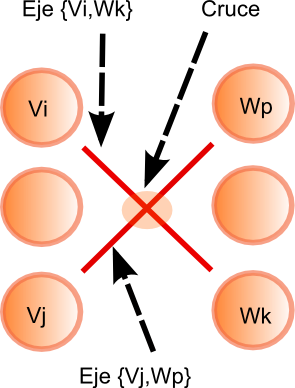
\includegraphics[scale=0.3]{./figuras/cruces/cruce.png}
     \caption{esquema de un cruce}
     \label{unCruce}
\end{figure}

Podemos entonces caracterizar en que casos se producen cruces:\\
\textit{Dado un orden de los nodos $p_1=<v_1,v_2,...,v_n>$ en una partici�n y un orden $p_2=<w_1,w_2,...,w_q>$ en la otra partici�n , se produce un cruce si existen ejes $(v_i,w_j)$, $(v_k,w_p)$ tal que $i<k \wedge p<j$.}

De esta manera un primer algoritmo para contar los cruces, consiste en tomar cada par de ejes y comparar las posiciones relativas de sus nodos.
Hacer esto tiene un costo $\theta(m^2)$, siendo $m$ la cantidad de ejes, ya que la cantidad de posibles pares de ejes es $\binom{m}{2} = \frac{m*(m-1)}{2}$. Este costo puede ser excesivo, principalmente en grafos densos, donde m puede ser del orden de $n_1*n_2$, siendo $n_i$ la cantidad de nodos en las particion i.

Buscamos entonces alg�n algoritmo que nos de un orden mejor que $O(m^2)$\footnote{cuando hablamos de complejidad en el �mbito del conteo de cruces, nos referimos a complejidad en el modelo uniforme}. 

Si se ordenan los ejes del grafo primero por su componente en la particion $p_1$ y luego por su componente $p_2$, es decir si $e_i=(i_1,i_2)$ y $e_j=(j_1,j_2)$ son ejes del grafo, consideramos que $e_i < e_j \Leftrightarrow i_1 < j_1 \vee (i_1 == j_1 \wedge i_2 < j_2)$ y consideramos luego el orden en el que quedan las segundas componentes, podemos ver que cada inversi'on es un cruce. Una inversi�n en el orden $\pi=<a_1,a_2,....a_n>$ es un par $(a_i,a_j)$ tal que $a_i > a_j$ $\wedge$ $i<j$. 

Decimos que una inversi�n representa a un cruce porque como primero se ordena por la primer componente (en verdad es la componente de la primer partici�n, pero para simplificar la notaci�n nos referiremos a dicha componente como la primer componente) y luego por la segunda, si hay una inversion es porque para los ejes $(v_k,a_i)$ y $(v_p,a_j)$ val�a que $v_k < v_p \wedge a_i > a_j$, y esa es la condici�n para que se produzca un cruce.

%TODO: ver si no hay q explicar mejor como se puede calcular eso
Entonces si ordenamos los ejes de esa manera y despu�s contamos las inversiones, podemos obtener el numero de cruces. Para ordenar a los ejes se puede utilizar radix sort, suponiendo que los ejes tienen como componentes las posiciones relativas de los nodos (o que estas se pueden obtener), lo cual se puede calcular en caso de que esa informaci�n no este disponible con un costo de $n_1 + n_2 + m $, con $n_i$ la cantidad de nodos de la partici'on i, obteniendo los indices de los nodos en cada particion y luego usando esta informaci�n ``traducir'' los ejes; y luego consideramos el arreglo que tiene a las segundas componentes de los ejes como elementos, aplicar insertion sort y por cada cambio de posici�n que se hace para un elemento, contar una inversi�n y por lo tanto un cruce. Esto �ltimo tendr�a un costo $O(m+c)$, con c la cantidad de cruces. En el peor caso, todos los ejes se cruzan por lo que tendr�amos un costo $O(m^2)$ nuevamente.

Veamos un ejemplo de como funciona este algoritmo:
Consideremos el siguiente grafo bipartito:
\begin{figure}[H]
    \centering
     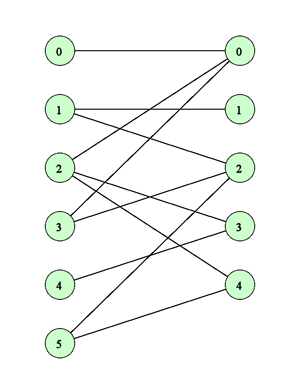
\includegraphics[scale=0.8]{./figuras/cruces/ejemplo1.png}
     \caption{Grafo de ejemplo para la aplicacion de los algoritmos de conteo de cruces}
     \label{ejemplo1}
\end{figure} 

Ahora ordenamos los ejes de acuerdo a su primer componente y luego a su segunda, obtenemos lo siguiente:

$$\left\langle (0,0),(1,1),(1,2),(2,0),(2,3),(2,4),(3,0),(3,2),(4,3),(5,2),(5,4)\right\rangle$$

Entonces el arreglo formado por las segundas componentes es el siguiente:

$$\left\langle0,1,2,\textcolor{Red}{0},3,4,0,2,3,2,4\right\rangle$$

Entonces, aplicamos selection sort. El 0 (de color rojo),recorre dos posiciones antes de insertarse en su posici�n correcta.

$$\left\langle0,0,1,2,3,4,\textcolor{Red}{0},2,3,2,4\right\rangle$$

Luego el tercer 0 se swapea cuatro veces:
 
$$\left\langle0,0,0,1,2,3,4,\textcolor{Red}{2},3,2,4\right\rangle$$

El segundo 2 cambia dos veces de posici�n:

$$\left\langle0,0,0,1,2,2,3,4,\textcolor{Red}{3},2,4\right\rangle$$

Ahora el segundo 3 cambia una vez de posici�n:

$$\left\langle0,0,0,1,2,2,3,3,4,\textcolor{Red}{2},4\right\rangle$$

Finalmente el �ltimo 2 es swapeado tres posiciones.

Entonces la cantidad de cruces del grafo es: $2+4+2+1+3 = 12$

Si bien en el caso general este algoritmo tiene un mejor orden, en peor caso sigue siendo $O(m^2)$.

Veamos un tercer acercamiento al problema: Sea $\sharp v_2$ la cantidad de nodos de la particion 2. Consideremos un arbol binario con $2^k$ hojas donde k es tal que $2^{k-1} < \sharp v_2 <= 2^{k}$ de modo de que cada nodo este en una hoja (podria haber hojas que no tengan a ningun nodo), dispuestos de izquierda a derecha seg�n su orden en la partici�n. Este �rbol tiene $2^{k+1}-1$ nodos. Ademas $k=\left\lceil log_{2}(\sharp v2)\right\rceil$

Lo que vamos a hacer es ordenar a los ejes como lo hicimos para el algoritmo anterior. Luego lo que haremos es agregar a los ejes segun dicho orden. Agregar el eje consiste en incrementar en uno el contador, en principio inicializado en 0, de la hoja correspondiente al nodo de la segunda componente del eje. Ademas se incrementa tambi�n en uno el contador del padre de dicha hoja y este incremento se va propagando hacia arriba hasta la ra�z.

Cada vez que insertamos un eje, en cada nivel, si estamos parados en un nodo izquierdo aumentamos el n�mero de cruces seg'un el valor del hermano del nodo.

El procedimiento puede resultar confuso en un principio por lo cual mostraremos un ejemplo de su aplicaci�n.
Apliquemos el algoritmo para el grafo de \ref{ejemplo1}:

Como tenemos $\sharp v_2 = 5$, el arbol va a tener 8 hojas y un total de 15 nodos.
 
\begin{figure}[H]
    \centering
     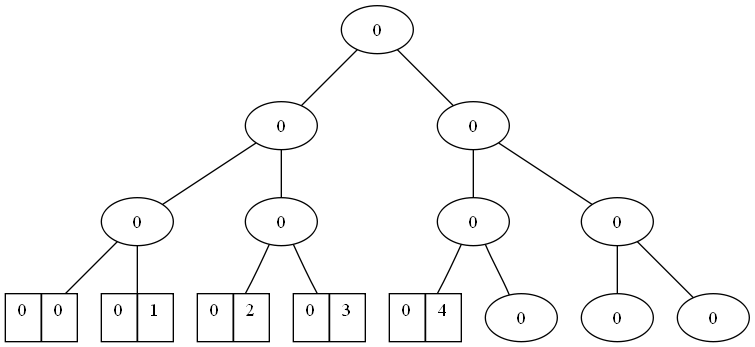
\includegraphics[scale=0.4]{./figuras/cruces/arbol.png}
     \caption{�rbol para contar cruces en el grafo de ejemplo}
     \label{arbol}
\end{figure} 

Los nodos cuadrados (del 'arbol) son las hojas que representan al nodo (del grafo bipartito) cuyo numero es el de la derecha de la hoja. Cada nodo tiene un contador , en principio inicializado en 0. El contador de cruces tambi�n esta inicializado en 0.

Recordemos que luego de ordenar los ejes el vector era:
$$\left\langle(0,0),(1,1),(1,2),(2,0),(2,3),(2,4),(3,0),(3,2),(4,3),(5,2),(5,4)\right\rangle$$

Lo primero que hacemos entonces es insertar el eje (0,0), de modo que se incrementa el contador de la hoja 0 y este incremento se propaga hacia arriba. Como 0 esta en un nodo izquierdo, lo que se hace es sumar a la cantidad de cruces el valor del contador del hermano de 0 (la hoja 1). Esto porque, porque el valor de dicho contador indica la cantidad de ejes insertados que terminaban en 1, pero ademas dado el orden que se usa para agregar a los nodos, sabemos que la primer coordenada de estos ejes que terminaban en 1 era menor que la del ejes que estoy insertando ahora, por lo tanto hay un cruce. En otras palabras, agregue un eje (a,1) antes que uno (b,0) y por como estban ordenados los nodos, sabemos que $a<b$ y como $1>0$, hay una inversi�n.

Al subir de nivel, como tambi�n estamos en un nodo izquierdo, agregamos a la cantidad de cruces el valor del contador del hermano correspondiente. En este caso, dicho contador guarda la cantidad de ejes agregados que terminan en 2 0 3. Y asi sucesivamente hasta la ra�z. 

Luego de esta inserci�n obtenemos el siguiente �rbol:
\begin{figure}[H]
    \centering
     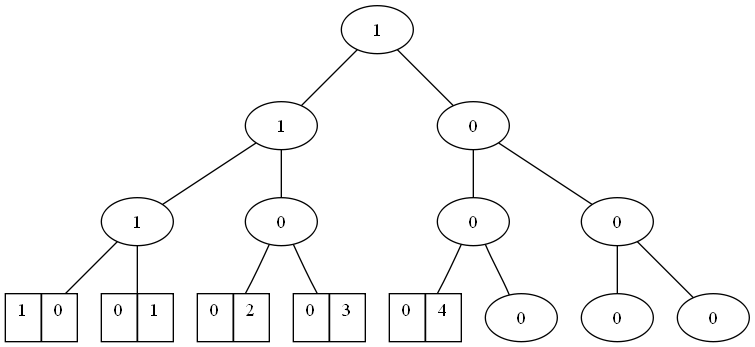
\includegraphics[scale=0.4]{./figuras/cruces/arbol2.png}
     \caption{�rbol con el eje (0,0) insertado}
     \label{arbol2}
\end{figure} 

De manera analoga, se insertan los ejes (1,1) y (1,2), sin que se generen cruces, en este caso el arbol queda de la siguiente manera:

\begin{figure}[H]
    \centering
     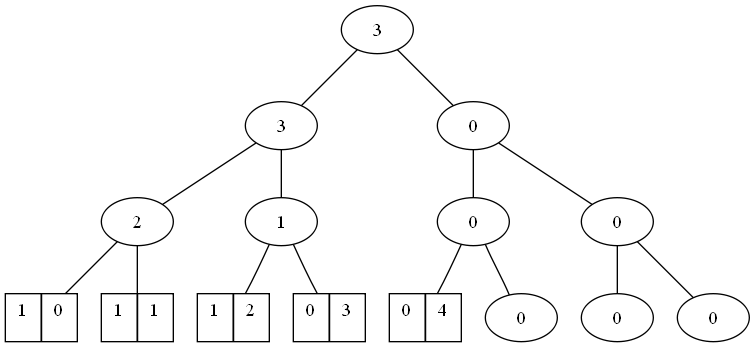
\includegraphics[scale=0.4]{./figuras/cruces/arbol3.png}
     \caption{�rbol con los ejes (0,0),(1,1) y (1,2) insertados}
     \label{arbol3}
\end{figure} 

Luego corresponde insertar el eje (2,0). Incrementamos en uno el contador de la hoja 0. Como es un nodo izquierdo, sumamos a cantidad de cruces el valor de la hoja 1, que es 1. Este incremento corresponde al cruce del eje (2,0) con el eje (1,1). Subimos un nivel e incrementamos en 1 el contador del padre de la hoja 0. Nuevamente sumamos al contador de cruces, el valor del contador del hermano del nodo donde estamos parados, ya que otra vez estamos en un nodo izquierdo. Este nuevo incremento corresponde al cruce entre el eje (2,0) y el eje (1,2). Seguimos subiendo hasta llegar a la ra�z, incrementando el valor de los contadores y en el caso de pasar por un nodo izquierdo, sumando el valor de los contadores de los nodos derechos. En particular en este caso, volvemos a caer en un nodo izquierdo, pero el contador de su hermano es 0. Esto se debe a que todavia no insertamos ning�n eje que terminara en 4.

\begin{figure}[H]
    \centering
     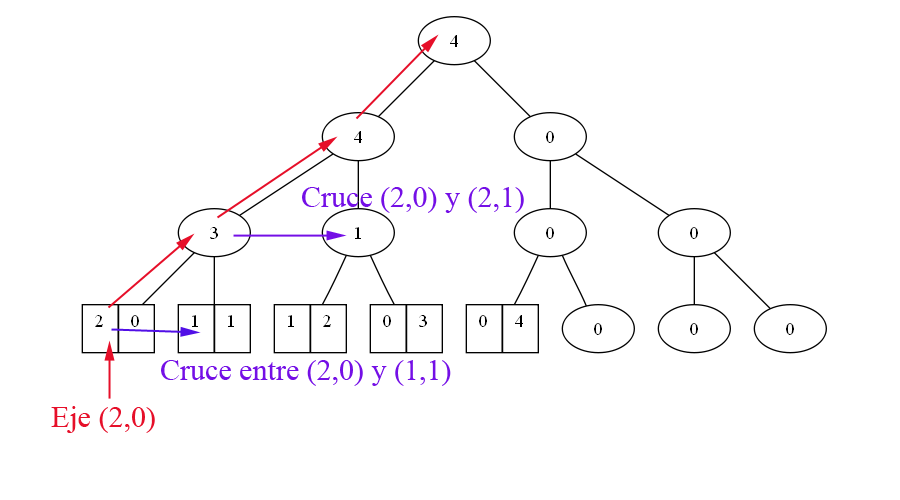
\includegraphics[scale=0.4]{./figuras/cruces/arbol4.png}
     \caption{�rbol con los ejes (0,0),(1,1),(1,2) y (2,0) insertados}
     \label{arbol4}
\end{figure} 


El procedimiento se repite hasta colocar todos los ejes.

Como veremos mas adelante, este procedimiento tiene como orden $O(max(m,\sharp v_1, \sharp v_2)+m*log(min_{i=1,2}(\sharp(v_i))))$

Repasando tenemos 3 algoritmos para calcular los cruces:
\begin{itemize}
\item El primero, consiste en revisar todo par de ejes. Tiene un costo $O(m^2)$
\item El segundo ordena los ejes y luego realiza insertion sort para contar inversiones. Tiene un costo de $O(max(m,\sharp v_1, \sharp v_2)+c)$
\item El tercero utiliza el arbol binario para contar inversiones. Tiene un orden $O(max(m,\sharp v_1, \sharp v_2)+m*log(min_{i=1,2}(\sharp(v_i))))$
\end{itemize}

Todas estos algoritmos requieren conocer el ``orden'' de los nodos en cada particion, lo cual podria hacerse, en $O(\sharp(v_1) + \sharp(v_2))$ costo que se suma a los algoritmos en caso de que no se tenga dicha informaci�n.

Si $m > log(min_{i=1,2}(\sharp(v_i)))$ conviene utilizar el tercer algoritmo, pues tiene una complejidad menor que la de los otros dos.

Si en cambio $m < log(min_{i=1,2}(\sharp(v_i)))$ (un grafo con muy pocos ejes) resulta conveniente utilizar el segundo algoritmo ya que provee un mejor orden.

Sin embargo, podemos evitar los casos donde se tengan pocos ejes. Para hacerlo, preprocesamos el grafo, de modo de sacar los nodos aislados, ya que estos se pueden insertar en cualquier lado sin que agreguen cruces.En el caso de un nodo del grafo original, si bien no puede insertarse en cualquier lado en el sentido estricto, vale que no suma cruces igualmente, por lo cual se lo puede sacar para aplicar cualquier algoritmo y luego insertarlo en la soluci�n en una posici�n valida.

De esta manera, el algoritmo 3 se muestra como la mejor opci�n, ya que si $m>\sharp v_i$, resulta que $O(max(m,\sharp v_1, \sharp v_2)+m*log(min_{i=1,2}(\sharp(v_i)))) \subseteq O(m*log(min_{i=1,2}(\sharp(v_i))))$.

\subsubsection{Pseudocodigo}
\begin{algorithm}[H]
\caption{Cuenta los cruces en un dibujo usando un arbol acumulador}
\begin{algorithmic}[1]
\PARAMS{particiones del dibujo (suponemos para simplificar que p2 tiene menos nodos (o igual cantidad) que p1)}
\PARAMS{los ejes del dibujo,las posiciones (indice) de los nodos}
\STATE ejsPorPos $\leftarrow$ $[]$
\FOR{cada eje(x,y) del dibujo}
\STATE agregar a ejesPorPos la tupla (posicion de x, posicion de y)
\ENDFOR
\STATE lista $\leftarrow$ RadixSort de los ejes de ejesPorPos de modo que (x,y) $<$ (z,w) si $x < z \vee x = z \wedge y < w$
\STATE primerIndice $\leftarrow$ $2^{ \left\lceil log_{2}(largo de p2) \right\rceil }$
\STATE arbol $\leftarrow \underbrace{[0,...,0]}_{2*primerIndice - 1}$
\STATE \COMMENT{arbol es el arbol acumulador}
\STATE decrementar primerIndice
\STATE cruces $\leftarrow$ 0
\FOR{cada eje de la lista}
\STATE indice $\leftarrow$ segunda componente del eje + primerIndice
\STATE arbol[indice] $\leftarrow$ arbol[indice] + 1 \COMMENT{un eje mas en esta hoja}
\WHILE{ indice $>$ 0}
\IF{indice es impar}
\STATE \COMMENT{estoy en un nodo izquierdo}
\STATE cruces $\leftarrow$ cruces + arbol[indice]
\ENDIF
\STATE indice $\leftarrow$ $(indice -1)/2$ \COMMENT{subo un nivel}
\STATE arbol[indice]~$\leftarrow$ arbol[indice] + 1
\ENDWHILE
\ENDFOR
\RETURN cruces
\end{algorithmic}
\end{algorithm} 

\subsection{Calculo de complejidad}
Sea $v_i$ la cantidad de nodos de la particion i, y m la cantidad de ejes del grafo.

Si bien comentamos que la funci�n podr�a en caso de que no este disponible calcular los indices de los elementos, esta funcionalidad no fue utilizada, de modo que el algoritmo recibe los indices ya armados. De este modo, el costo de armar y manter a los indices sera tenido en cuenta en los respectivos algoritmos que utilicen a esta funci�n.

Primero lo que hacemos es traducir los ejes, segun los indices. Para hacer esto, lo que se hace es recorrer todos los ejes (se recorren las listas de adyacencia de los nodos de una de las particiones) y se van guardando en una lista, los ejes con sus compoentes traducidas (ciclo de la l�nea 2).

Luego ordenamos los ejes, como lo hacemos con radix sort, el costo es $max(m, v_1, v_2)$, puesto que tengo que ordenar m ejes, y para hacerlo voy a necesitar de $\sharp v_1$ $buckets$ primero y $\sharp v_2$ $buckets$ luego.

Una vez ordenado y armado el 'arbol, que se puede hacer en O($v_2$) como se vera mas adelante, vamos a mirar todos los ejes. Para cada eje recorremos el arbol desde una hoja hasta la raiz. Como el arbol tiene $2^k$ hojas, tiene $log_{2}(2^k)$ de altura, pero $log_{2}(2^k)=k=\left\lceil log_{2}(\sharp v2)\right\rceil$.

El arbol se puede implementar sobre un arreglo, de modo que la posici�n 0 sea la ra�z, la 1 y 2 sus hijos izquierdo y derecho respectivamente, y asi sucesivamente (de manera analoga a como se hace para implementar un heap). De esta manera, los nodos izquierdos del �rbol quedan en las posiciones impares, y aumentar cada contador, asi como tambi�n moverse dentro del �rbol de un nodo a su padre se puede hacer en O(1). Por lo tanto, el costo de insertar todos los ejes es $O(max(m,\sharp v_1, \sharp v_2)+m*log(\sharp v_2) )$.

\begin{figure}[H]
    \centering
    \subfigure[�rbol acumulador]{
     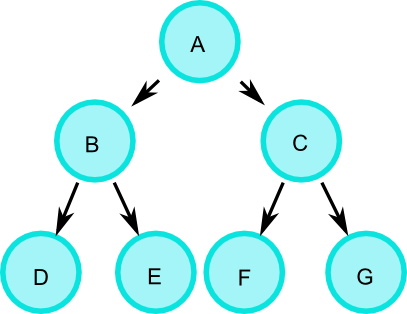
\includegraphics[scale=0.2]{./figuras/cruces/arbolito.png}}
     \subfigure[Representaci�n en arreglo]{
     
\includegraphics[scale=0.2]{./figuras/cruces/arreglito.png}}

\end{figure} 

Ahora bien, en vez de ordenar primero por la primer componente y luego con respecto a la segunda, podr'iamos hacer el mismo procedimiento pero ordenando primero por la segunda, luego por la primera y armando el arbol para $v_1$. Entonces, en particular el procedimiento se podria realizar utilizando el  $v_i$ de menor cardinal. Con lo cual el costo de las inserciones es de $O(max(m,\sharp v_1, \sharp v_2)+m*log(min_{i=1,2}(\sharp v_i) ))$

Como dijimos, este algoritmo podria no ser eficiente si la cantidad de ejes es muy peque�a, ya que para hacer radix sort se van a recorrer todos los nodos de ambas particiones, lo cual podria ser un costo mas grande que mirar todos los ejes. Sin embargo, tambi�n comentamo que vamos a filtrar a los nodos de grado 0 antes de trabajar con el dibujo, por lo cual creemos que este algoritmo es eficiente. Filtrar a los nodos de grado 0 tiene sentido, ya que por ejemplo en nuestro algoritmo exacto, un peque�o incremento en la cantidad de nodos, siginifica un gran aumento en la cantidad de permutaciones, de esta manera si lo separamos el algoritmo no perderia tiempo en mover a este nodo que no genera cambio alguno.

\subsection{Reutilizaci�n de los c�lculos}
\label{reUso}
Si bien hay situaciones donde el orden relativo de los nodos en las particiones se podr�a modificar sustancialmente, por lo cual ser�a necesario recalcular los cruces nuevamente , lo cual, como vimos en la secci�n anterior, tiene un costo bastante alto; hay otros casos donde se hace una modificaci�n mas peque�a al orden de los mismos y es posible no recalcular todos los cruces.

En particular si tenemos un orden de los nodos $\pi=\left\langle v_1,v_2,...v_i,v_{i+1},...,v_n \right\rangle$ y realizamos un ``swap'' entre dos posiciones consecutivas $i$, $i + 1$, podemos observar que si $\pi_1=C(\left\langle v_1,v_2,...,v_{i+1},v_{i},...v_n \right\rangle$ y definimos C($\pi$,$\rho$) como la cantidad de cruces entre los ejes del grafo, dado que los nodos de la primer partici�n estan ordenados seg'un $\pi$ y los de la segunda segunda seg�n $\rho$, vale que:

 $$C(\pi_1,\rho) = C(\pi,\rho) - CrucesEntre(v_i,v_{i+1},\rho) + CrucesEntre(v_{i+1},v_i,\rho)$$

Donde CrucesEntre(a,b,$\rho$) es la cantidad de cruces entre ejes de $a$ y ejes de $b$ si $a$ esta en una posicion relativa menor que la de $b$ y dado que los nodos de la otra partici�n estan en el orden $\rho$. Esto se debe a que como dijimos anteriormente, los cruces dependen solo del orden relativo. Entonces si intercambiamos dos posiciones consecutivas, el orden relativo de los demas nodos se mantiene, es decir, los que estaban ``abajo'' de ellos siguen estando all�, y los que estaban ``arriba'' tambi�n, de modo que solo cambian los cruces que hay entre los dos nodos movidos.

\begin{figure}[H]
    \centering
    \subfigure[]{
     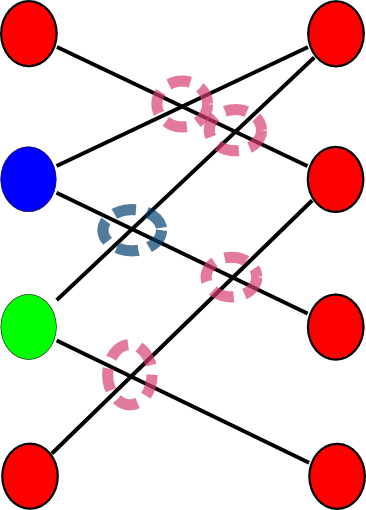
\includegraphics[scale=0.2]{./figuras/cruces/crucesPreSwap.png}}
     \subfigure[]{
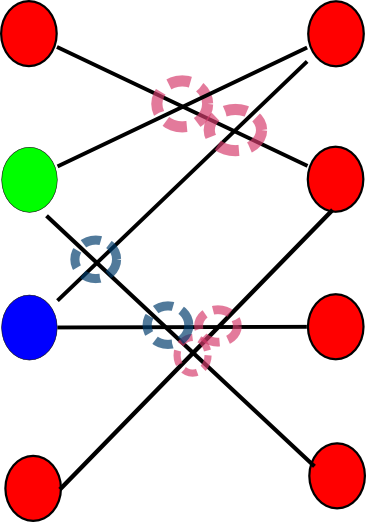
\includegraphics[scale=0.2]{./figuras/cruces/crucesPostSwap.png} }
     \label{fig:swap}
     \caption{Al intercambiar los nodos verde y azul, los cruces que involucran al resto de los nodos se mantienen}
\end{figure} 


Para calcular crucesEntre se puede utilizar el algoritmo antes descripto para el conteo de cruces en general, simulando una partici�n que solo contenga a los nodos $a$ y $b$, y solo teniendo en cuenta los ejes que salen de ellos dos. En este caso, como la partici�n mas chica tiene 2 nodos (o menos si una partici�n era solo un nodo), resulta que el algoritmo puede calcular los cruces en $O( v_j + m_{a} + m_{b})$ con $m_{a,b}$ la cantidad de ejes incidentes a $a$ y a $b$ y $v_j$ es la otra partici�n. Basicamente lo que hacemos solo mirar los ejes que salen de a y de b, armar un arbol de dos posiciones y aplicar el procedimiento anterior

%FIXME: Esto esta bien?
En el caso en que a y b tengan pocos ejes, de modo tal que $m_{a}*m_{b} < \sharp v_j$ , utilizamos la versi�n simple del algoritmo toma todos los pares de ejes de a y b. De este modo el orden para contar cruces es $min(max(v_j,m_a,m_b),m_a*m_b)$
 
\begin{figure}[H]
    \centering
    \setcounter{subfigure}{0}
    \subfigure[]{
     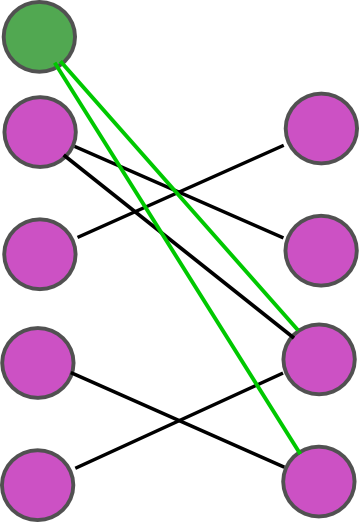
\includegraphics[scale=0.2]{./figuras/cruces/nuevoNodo.png}}
     \subfigure[]{
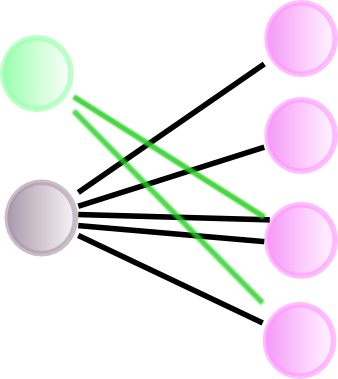
\includegraphics[scale=0.2]{./figuras/cruces/compactado.png} }
     \caption{Compactaci�n del grafo para averiguar cuantos cruces agrega un nuevo nodo}
     \label{fig:compactar}
\end{figure} 

Otro caso donde se puede evitar re calcular todos los cruces es cuando se agrega un nodo al dibujo, particularmente si se agrega al principio o al final de la partici�n. En este caso, los cruces existentes entre otros nodos se mantienen, solo se podr�an agregar nuevos cruces con los ejes del nodo recien agregado. Entonces podemos colapsar los nodos de la partici�n donde se esta agregando el nuevo nodo, dejando solo al nuevo nodo y a un nodo $w$ con todos los ejes del resto como ilustra la figura \ref{fig:compactar}, de modo de que el algoritmo sea $O(m + v_1+v_2 + m)$. Esto es asi porque el costo de la traducci�n y del radix sort hay que hacerlo igual, pero al igual que en el caso de los cruces entre dos nodos consecutivos, el arbol tiene solo 2 elementos: el nodo que se agrega y el nodo que compacta a todos los demas con sus ejes.

Estas situaciones si bien parecen casos muy especificos, pueden ser aprovechados por los distintos algoritmos que desarrollamos.

\section{Eliminaci�n de nodos nulos}
\label{sacoNulos}
Como dijimos, antes de aplicar las heuristicas, eliminamos los nodos de grado cero en lo que ser�a el grafo con todos los nodos ya puesto. Consideramos que esto evita que las heuristicas, asi como tambi�n el algoritmo exacto, realicen calculos innecesarios.

Para hacerlo, basicamente tomamos los nodos de la entrada, asi como sus ejes y construimos un dibujo. A partir de este dibujo, que ya tiene armadas las listas de adyacencia, podemos separar en una lista a los nodos de grado distinto a cero. 

\begin{figure}[H]
    \centering
    \setcounter{subfigure}{0}
    \subfigure[]{
     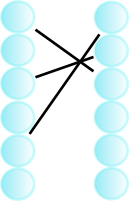
\includegraphics[scale=0.2]{./figuras/cruces/pocosEjes.png}}
     \subfigure[]{
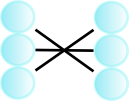
\includegraphics[scale=0.2]{./figuras/cruces/limpio.png} }
     \caption{Reducir la cantiidad de cruces en el primero es equivalente a hacerlo en el segundo}
     \label{fig:limpieza}
\end{figure} 

Si solamente los sacaramos, nos encontrar�amos frente al problema de que los nodos no tienen como identificadores n�meros consecutivos. Por esta raz�n, no solo filtramos a los nodos de grado nulo, sino que se realiza un nueva n�meraci�n de los nodos que quedan. La misma cumple que los nodos fijos tienen n�meraci�n consecutiva (la cual ademas indica la posici�n relativa, es decir si a $<$ b con a y b nodos de la misma partici�n, entonces el nodo fijo a esta antes que el nodo fijo b) y que los n�meros son asignados primero a los nodos fijos de la primer partici�n, luego a los nodos fijos de la segunda, en tercer lugar a los nodos no fijos de la primera y finalmente a los de la segunda.

Para realizar dicha traducci�n se utilizan diccionarios sobre arreglos a fin de poder realizarla rapidamente. Lo que se guarda es dado un identifador nuevo a que nodo viejo identifica. 

Los ejes tambi�n son traducidos, por lo cual se necesita momentaneamente poder ir de un identificador viejo a su numero nuevo, por lo cual se necesita otro indice provisioriamete.

Una vez que se realiz� la traducci�n, las heuristicas y el algoritmo exacto trabajan con el dibujo nuevo.

Cuando terminan se realiza el proceso inverso para volver de los nodos nuevos a los viejos, y ademas insertar a los viejos en posiciones validas (hay que respetar la posicon de los nodos fijos que ten�an grado cero y no fueron tenidos en cuenta)

Todo este proceso nos agrega un costo $O(V_1+V_2+m)$ donde $V_i$ es la cantidad de nodos de partici�n i sin filtrar y m la cantidad de ejes. En el peor caso, ning�n nodo ten�a grado cero, por lo que esta mejora representa un overhead, sin embargo como se ver� mas adelante el orden de los distintos algoritmos es lo suficientemente elevado como para hacer despreciable dicho overhead.

%TODO: comparar que pasa si no saco los nodos al pedo y si los saco

\chapter{Algoritmo exacto}
\section{Desarrollo}
Un dibujo incremental v�lido consiste en una permutaci�n de los nodos 
de cada partici�n que mantenga el orden relativo de los nodos previamente 
fijados. Dados $v_i$ nodos originales en la partici�n i, se agregan $IV_i$ 
nodos en cada partici�n. La cantidad posible de soluciones es:
$$IV_1!*\dbinom{IV_1 + v_1}{v_1}*(IV_2!*\dbinom{IV_2 + v_2}{v_2})$$
Esto se debe a que la partici�n 1 tiene $IV_1 + v_1$ nodos, y por lo 
tanto hay esa cantidad de posiciones. De esas, $v_1$ estar�n destinadas a los
nodos existentes, cuyo orden relativo es fijo. Una vez que elegimos sus posiciones, 
el orden entre ellos es fijo. En las $IV_1$ posiciones restantes podemos poner 
cualquier permutaci�n de los nodos nuevos. Luego la cantidad de �rdenes v�lidos
para la partici�n 1 es: 
$$ IV_1!*\dbinom{IV_1 + v_1}{v_1} $$
Luego, para cada uno de estos �rdenes v�lidos en la partici�n 1, tenemos (an�logamente)
una cantidad equivalente para la partici�n 2:
$$IV_2!*\dbinom{IV_2 + v_2}{v_2}$$ permutaciones en la segunda partici�n.
El total de combinaciones es finalmente el producto de las combinaciones de cada
partici�n, que resulta en la f�rmula presentada anteriormente.

Dada la naturaleza exponencial del problema a resolver, decidimos utilizar la t�cnica de
\textit{backtracking} para formular un algoritmo exacto. Comenzamos por desarrollar un algoritmo
de fuerza bruta que simplemente explora el �rbol de combinaciones que va generando progresivamente,
y luego lo fuimos refinando agregando optimizaciones y podas.

El algoritmo de backtracking aprovecha la naturaleza recursiva del problema de dibujo incremental,
agregando progresivamente cada nodo m�vil en todas sus posiciones v�lidas y produciendo as�
un nuevo conjunto de nodos fijos que se incrementar� con una llamada recursiva. Dado un candidato
inicial con una cantidad de cruces dada, esta situaci�n nos permite realizar una poda sencilla
del �rbol de combinaciones. Ocurre que inevitablemente todo dibujo incremental del grafo parte
de un dibujo original cuya cantidad de cruces acota inferiormente la del dibujo incrementado.
Por lo tanto, al construir un candidato para una llamada recursiva, si la cantidad de cruces
en su parte fija supera a la del mejor candidato hallado hasta el momento, no tiene sentido descender
por la rama y puede podarse sin perder soluciones.

Con esta idea, resulta �til proveerse r�pidamente de un candidato inicial cuya cantidad de cruces
sea baja, ya que \textit{a priori} permitir� descartar mayor cantidad de ramas por pasarse de su
valor. Con este fin, tiene sentido utilizar alguna soluci�n heur�stica de las desarrolladas en este
trabajo.

El pseudoc�digo del algoritmo resultante es aproximadamente:
\begin{algorithm}[H]
\caption{Halla la soluci�n exacta al problema de dibujo bipartito incremental}
\begin{algorithmic}[1]
\PARAMS{fijo1, fijo2, movil1, movil2, adyacencias}
\STATE construir un candidato abritrario y 
\IF{fijo1 = $\emptyset$ y fijo2 = $\emptyset$}
    \IF{el dibujo obtenido tiene menos cruces que el mejor candidato}
        \STATE reemplazar el mejor candidato por este dibujo
    \ENDIF
\ELSIF{fijo1 $\neq$ $\emptyset$}
    \STATE tomar el primer elemento de movil1
    \FOR{cada posici�n del elemento en fijo1}
        \STATE poner el elemento en esa posici�n
        \IF{el dibujo obtenido no tiene m�s cruces que el mejor candidato}
            \STATE llamar recursivamente
        \ENDIF
        \STATE sacar el elemento de esa posici�n
    \ENDFOR
\ELSIF{fijo2 $\neq$ $\emptyset$}
    \STATE tomar el primer elemento de movil2
    \FOR{cada posici�n del elemento en fijo2}
        \STATE poner el elemento en esa posici�n
        \IF{el dibujo obtenido no tiene m�s cruces que el mejor candidato}
            \STATE llamar recursivamente
        \ENDIF
        \STATE sacar el elemento de esa posici�n
    \ENDFOR
\ENDIF
\RETURN el mejor candidato hallado
\end{algorithmic}
\end{algorithm}

De esta manera, el �rbol de \textit{backtracking} que tenemos es:
\begin{figure}[H]
\centering
\setcounter{subfigure}{0}
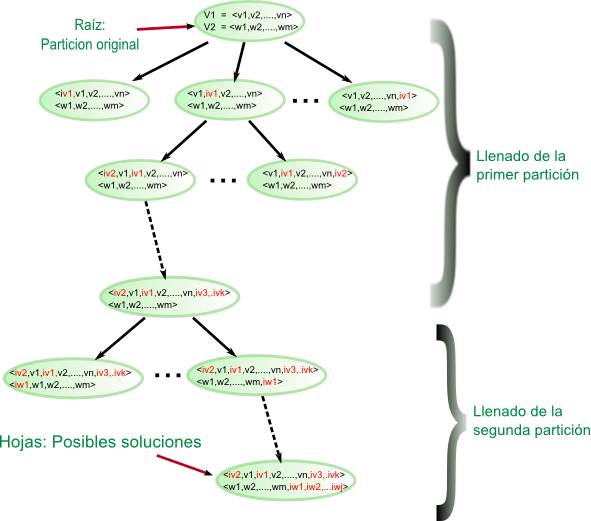
\includegraphics[scale=0.9]{./figuras/exacto/arbolbt.png}
\caption{�rbol de \textit{backtracking}}
\end{figure}

El algoritmo lo recorre en orden DFS, cortando aquellas ramas que pueden ser descartadas
inmediatamente sin visitarlas.

\subsection{Implementaci�n eficiente}

Dado que el algoritmo recursivo se ejecutar� una vez por cada nodo del �rbol de combinaciones,
es importante que su ejecuci�n sea lo m�s eficiente posible para disminuir el tiempo total
de ejecuci�n.

La primera versi�n del algoritmo era similar a la de fuerza bruta: recorr�a el �rbol de combinaciones,
y cuando obten�a una permutaci�n completa, constru�a el dibujo y contaba enteramente sus cruces.
A continuaci�n agregamos la poda simple descripta anteriormente. Sin embargo, resultaba claro
que recalcular los cruces de todo el dibujo para cada hoja del �rbol de permutaciones no era
eficiente ya que gran parte de los c�lculos eran redundantes entre hojas vecinas del �rbol, puesto
que compart�an gran parte de las posiciones de los nodos en el dibujo.

Utilizando los m�todos descriptos anteriormente, decidimos efectuar los c�lculos mediante
una t�cnica incremental. Constatamos que la iteraci�n que en el pseudoc�digo corresponde
a agregar un nodo m�vil en todas las posiciones posibles dentro del dibujo fijo de su partici�n
puede describirse en t�rminos de 3 operaciones: agregar el nodo al final del dibujo, 
permutarlo $n$ veces hacia atr�s con su vecino inmediato, y finalmente extraerlo del principio 
del dibujo donde habr� quedado ubicado. Con este procedimiento, un nodo m�vil dado
pasa por todas las posiciones posibles dentro del dibujo fijo original.

\begin{figure}[H]
\centering
\setcounter{subfigure}{0}
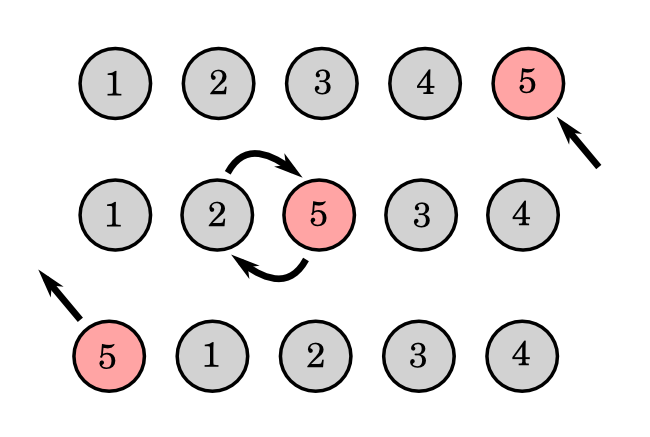
\includegraphics[scale=0.25]{./figuras/exacto/swaps.png}
\caption{Permutaciones mediante swaps}
\end{figure}

Dado un candidato, la cantidad de cruces que se agregan por agregarle un nuevo nodo al 
final a una partici�n puede ser calculada mucho m�s r�pidamente que los cruces de todo 
el dibujo. Adem�s, como se vio anteriormente, calcular la cantidad de cruces que resulta
de un \textit{swap} tambi�n es eficiente. Esta mejora se incluye en el algoritmo evitando
as� recalcular todos los cruces para cada permutaci�n, y en cambio llevando una cuenta temporal
de cruces que se modifica continuamente para reflejar los cruces del candidato que se est�
evaluando.

\subsection{Tabulado de resultados}

A�n tras incluir los c�lculos incrementales como se describi� en el �ltimo p�rrafo, se puede
aprovechar de forma m�s eficiente a�n la realizaci�n de ciertos c�lculos.
Consideremos un dibujo con dos permutaciones $V = <v_1,v_2,...,v_n>$, $W = <w_1,w_2,...,w_k>$.
La cantidad de cruces puede obtenerse como:
$$Cruces(V,W) = \sum_{i=1}^{k-1}{\sum_{j=i+1}^{k}{crucesEntre(w_i,w_j,V)}}$$

Esto es, dada una permutaci�n de V, los cruces de todo el dibujo, para cualquier
permutaci�n de W, dependen �nicamente de los valores de $crucesEntre(w_i, w_j, V)$, funci�n
que calcula los cruces entre dos nodos $w_i$ y $w_j$ para la permutaci�n de V elegida y
suponiendo que $w_i$ est� antes de $w_j$ en el dibujo. Esto puede hacerse ya que la cantidad
de cruces que se producen entre los ejes de 2 nodos de una partici�n depende �nicamente de su
orden relativo y de las posiciones dentro de la partici�n restante.

Por lo tanto, una vez que construimos una permutaci�n de una de las 2 particiones (parte superior
del �rbol en el gr�fico explicativo del �rbol de \textit{backtracking}), podemos tabular los $k^2$
valores de  $crucesEntre()$ necesarios para el c�lculo de los cruces de cualquier permutaci�n de
la otra partici�n: todo el sub�rbol que pende de una permutaci�n completa de la partici�n 1 comparte
los mismos valores de $crucesEntre()$. Teniendo esta tabla, el c�lculo de cruces del dibujo completo
puede realizarse mediante la suma de los mismos seg�n la f�rmula de arriba, lo cual podr�a agilizar
el conteo de cruces. Cabe destacarse que el llenado de esta tabla tiene un costo no despreciable,
y por tanto es importante realizar pruebas para determinar si las ventajas de realizar este tabulado
no son superadas por el costo de la creaci�n de la tabla. 

Como se ver� m�s adelante, las pruebas mostraron que el uso de esta tabulaci�n mejora significativamente
el rendimiento del algoritmo. En funci�n de esta mejora, podemos observar que los c�lculos realizados
con ayuda de la tabla son mucho m�s r�pidos que los que se realizan sin ella. Por lo tanto decidimos
incluir una segunda mejora que consiste en decidir cual de las 2 particiones tiene m�s permutaciones
posibles, y asignar �sta a la parte inferior del �rbol cuya exploraci�n est� m�s optimizada gracias al
uso de la tabla. Antes de esta decisi�n, se tomaba de forma arbitraria que lo recibido como
``partici�n 1'' se ubicaba en la parte superior del �rbol, puesto que la situaci�n era sim�trica y solo
influ�a el tama�o total del �rbol.

Si bien no es posible realizar la misma tabulaci�n para la partici�n asignada a la parte
superior del �rbol (puesto que no disponemos de la ubicaci�n de los nodos en la otra partici�n
a�n), es posible realizar una optimizaci�n parcial: si bien no conocemos las posiciones
de \textit{todos} los nodos en la partici�n vecina, si conocemos la posici�n de aquellos
que son fijos y por tanto no modifican su orden relativo. Se puede construir una tabla m�s
peque�a para, nuevamente, agilizar el conteo de cruces en las permutaciones de la
partici�n de la parte superior.

\subsection{Podas}

Disponiendo de la tabla de cruces entre pares de nodos, pudimos construir una funci�n de poda
m�s efectiva, mediante una cota inferior m�s fina para la cantidad m�nima de ejes que produce
una rama. Nuevamente, para una permutaci�n dada de $V$, tenemos que:

$$Cruces(V,W) \geq \sum_{i=1}^{k-1}{\sum_{j=i+1}^{k}{min(crucesEntre(w_i,w_j,V),crucesEntre(w_j,w_i,V))}}$$

Como tenemos estos valores tabulados, resulta muy sencillo calcular esta cota y podar en funci�n
del valor obtenido. Esto utiliza el hecho de que dados dos nodos $w_i$, $w_j$ de la partici�n 2, 
una vez que se los coloque en el dibujo, agregar�n una cierta cantidad de cruces (ya sea $crucesEntre(w_i, w_j)$
o $crucesEntre(w_j, w_i)$ dependiendo de su orden relativo). Como disponemos de estos dos valores,
podemos usar el m�nimo entre ambos como una cota inferior de los cruces producidos por la dupla
$w_i$, $w_j$ dada la permutaci�n de $V$ tomada.

Una vez que tenemos esta cota inferior, podemos descartar de antemano a aquellas ramas donde el
valor de dicha cota supere la cantidad de cruces del mejor candidato obtenido hasta el momento.
Una vez m�s, este c�lculo redunda en un costo adicional que podr�a ser contraproducente
en caso de que la poda no lograra eliminar una cantidad significativa de ramas. Nuevamente, es
necesario realizar pruebas para determinar su efectividad. Las mediciones observaron que este
mecanismo de poda es particularmente bueno y elimina partes sustanciales del �rbol de permutaciones
sin un costo excesivo (producto, en gran parte, de la disponibilidad de la tabla de cruces
descripta previamente, que aligera mucho el c�mputo de la cota).


\section{Pseudoc�digo}
\begin{algorithm}[H]
\caption{Resuelve de forma exacta el problema de dibujo incremental de grafos bipartitos}
\begin{algorithmic}[1]
\STATE generar excepci�n de no implementado
\end{algorithmic}
\end{algorithm}

\section{Detalles de implementaci�n}
% uso de listas doblemente enlazadas para push_back(), pop_front() y swap() en O(1)

% uso de buffers �nicos para fijo1, fijo2, movil1, movil2 y cruces que son usados
% por todas las instancias recursivas del algoritmo (ahorra mucho espacio en stack y evita
% muchas copias de listas o conjuntos de nodos fijos y moviles).

% uso de diccionarios sobre arreglo para mayor velocidad (el uso de memoria del
% algoritmo est� b�sicamente determinado por el tama�o del stack, por lo tanto
% no tiene sentido optimizar el uso de memoria de los factores constantes)

% uso de la heur�stica constructiva para determinar el candidato inicial

\section{C�lculo de complejidad}
Antes de correr nuestro algoritmo exacto, lo que hacemos es limpiar el grafo, lo cual nos da un costo inicial $O(V_1+V_2+m)$ donde $V_i$ es la cantidad de nodos de partici�n i sin filtrar y m la cantidad de ejes.

Al iniciar lo que hacemos es inicializar ciertas variables que nos ser�n de utilidad tales como las listas de adyacencia parciales, vectores con posiciones, etc. Todo esto tiene un costo $O(v_1+v_2 + m)$ donde $v_i$ es la cantidad de nodos de una partici�n. Esto lo podemos acotar por  $O(v_max + m)$. En esta inicializaci�n se llena la tabla de resultados para la primer partici�n. Lo que calculamos es $crucesEntre(w_i,w_j) \forall w_i,w_j \in v_1$. Esto tiene un costo $O(v_{1}*v_{max})$, ya que son $O(v_{1})$ calculos y cada calculo tiene cosot $O(v_{max})$.
  %TODO: completar
Para realizar el estudio de este algoritmo creemos que ser� provechoso considerar por separado el llenado de cada partici�n. Como comentamos antes, primero se llena una de las particiones, y despu�s se llena la otra. Ademas consideraremos para el estudio el caso donde no es posible podar nada.

Primero observemos el costo que tenemos al pasar por cada nodo del arbol de permutaciones de la primer partici�n. En cada paso lo que hacemos es insertar un elemento al final, y contar cuantos cruces nos agrega, lo cual lo hacemos en $O(v_1+ m )$. Esto �ltimo no es cierto, pues en verdad no se inserta para cada nodo del �rbol, sino que dado un nivel, el elemento se inserta tantas veces como nodos hay en nivel anterior del arbol y luego se hace swap, sin embargo para no hacer mas engorroso aun el calculo, decidimos simplificarlo de esa manera. Luego intentamos aplicar la poda. Aplicarla tiene un costo $O(v_{1}^2)$ ya que tengo que obtener la suma de los minimos de los cruces entre dos elementos y dichos elementos ya estan en la tabla. Despu�s hacemos otra llamada para ir armando el siguiente nivel. Una vez que regresamos de esa llamada, hacemos un swap del nodo con un adyacente, y actualizamos los cruces, esta actualizaci�n la hacemos en $O(1)$ ya que tenemos los cruces entre ambos tabulados.

Entonces recorrer el �rbol de llenado de la primer partici�n tiene un costo:

$$O(nodos * (v_{1}^2 +(v_1+m)))$$

aqui nodos es la cantidad de nodos del arbol de permutaci�n. Veamos cuantos nodos tiene:
Podemos obtener la cantidad de nodos del arbol en funci�n de la cantidad de nodos moviles y fijos que tiene, de la siguiente manera:
%TODO: gonza explica esta formula
  \begin{equation}
     tamArbol(moviles,fijos) = \left\{
	       \begin{array}{ll}
		 1      & \mathrm{si\ } moviles = 0 \\
		(fijos+1)*tamArbol(moviles-1,fijos+1) + 1 & \mathrm{si\ } moviles \neq 0 \\
	       \end{array}
	     \right.
   \end{equation}

Esta formula no es facilmente manejable, por lo cual usaremos una cota. Dado que cada nivel tiene mas nodos que el nivel anterior (si tengo una permutaci�n de k elementos, al agregar un nuevo elemento obtenemos k + 1 posibles ordenes), podemos acotar la cantidad de nodos del arbol como:
 $$h*moviles_1!*\dbinom{moviles_1 + fijos_1}{fijos_1}$$

Donde h es la altura del arbol y $moviles_1!*\dbinom{moviles_1 + fijos_1}{fijos_1}$ es la cantidad de hojas.

La altura del �rbol es igual a la cantidad de nodos moviles en la partici�n 1, ya que en cada nivel estamos agregando un nodo, mas 1 por la raiz donde no agregamos nada todavia. Luego:

cantidad de nodos $\leq moviles_1*moviles_1!*\dbinom{moviles_1 + fijos_1}{fijos_1}$

Luego el orden de completar todas las permutaciones de la primer partici�n nos qued�:

$$O(moviles_1*moviles_1!*\dbinom{moviles_1 + fijos_1}{fijos_1}(v_1+m+v_{1}^2))$$

En cada hoja del arbol de las permutaciones de la primer partici�n, completamos la tabla para la segunda partici�n. Esto tiene un orden $O(v_2*v_{max})$

Completar la segunda partici�n tiene el mismo costo que completar la primer partici�n, con la salvedad de que en las hojas tenemos un costo $O(v_1+v_2)$ por copiar al mejor dibujo (el grafo no se copia, se usa una referencia).

Entonces, completar el arbol de la segunda particion tiene un costo:
$$O(moviles_2*moviles_2!*\dbinom{moviles_2 + fijos_2}{fijos_2}(v_2+m+v_{2}^2) + (v_1+v_2)*moviles_2!*\dbinom{moviles_2 + fijos_2}{fijos_2}(v_2+m+v_{2}^2))$$

Para cada hoja del arbol de la primer partici�n, llenamos todo un �rbol de la segunda. Por lo tanto el costo final es (luego de sacar algunos factores comunes):

%$ O(moviles_1*moviles_1!*\dbinom{moviles_1 + v_1}{v_1}(v_1+m+v_{1}^2) + moviles_1!*\dbinom{moviles_1 + v_1}{v_1}(v_1+m+v_{1}^2) *(moviles_2*moviles_2!*\dbinom{moviles_2 + fijos_2}{fijos_2}(v_2+m+v_{2}^2) + (v_1+v_2)*moviles_2!*\dbinom{moviles_2 + fijos_2}{fijos_2}(v_2+m+v_{2}^2))+\dbinom{moviles_1 + v_1}{v_1}(v_1+m+v_{1}^2)*v_2*v_{max})$

$O(moviles_1!*\dbinom{moviles_1 + v_1}{v_1}(v_1+m+v_{1}^2)*(moviles_1+ moviles_2!*\dbinom{moviles_2 + fijos_2}{fijos_2}(v_2+m+v_{2}^2)*(moviles_2 + (v_1+v_2)) + v_2*v_{max}) + V_1 + V_2)$ 

De la formula vemos que es preferible tomar como primer partici�n a aquella que tenga una menor cantidad de hojas, de esta manera la segunda tabla se construye menos veces y se aprovechan mas calculos.

\section{An�lisis experimental}

\subsection{Experiencias realizadas}
% utilidad de invertir particion1 y particion2
% aptitud de las podas: poda "simple" vs. poda loca
% utilidad de las tablas: algoritmo con y sin tabulado
% tiempos para un grafo con cantidad de permutaciones dadas y densidad de ejes variable
% tiempos del algoritmo de backtracking vs. tabla vs. tabla + poda loca (en funcion de las combinaciones)

\subsection{Resultados}
% estimaci�n del tiempo del algoritmo para resolver un caso dado (en funci� de la cantidad de combianciones)

\section{Discusi�n}

\chapter{Heur�sticas Constructivas}
\label{constructivas}


\section{Introducci�n}
Presentamos a continuaci�n tres diferentes ideas de heur�stica constructiva
para el problema de dibujo de grafo bipartito. Comentaremos las ideas detr�s
de cada una as� como un ejemplo de su aplicaci�n y el pseudoc�digo correspondiente,
para luego examinar emp�ricamente su comportamiento a partir de prototipos
en Python. Con esta informaci�n, elegiremos la de mejor comportamiento 
para su implementaci�n definitiva en C++, que ser� la que utilicemos
posteriormente en el algoritmo GRASP. Las heur�sticas utilizan los m�todos 
incrementales para conteo de cruces descriptos en \ref{reUso}.

En todos los casos se trata de heur�sticas \textit{greedy} que parten del
dibujo a incrementar y agregan progresivamente los elementos nuevos (nodos,
ejes o ambos) en la posici�n que optimiza alg�n criterio \textit{greedy}.

\section{Descripci�n de las heur�sticas}

\subsection{Heur�stica de inserci�n de nodos}

El primer enfoque que evaluamos consiste en partir del dibujo original (aquel
cuyos nodos est�n en un orden que no puede ser alterado) y se completa progresivamente
agregando los nodos nuevos en la posici�n �ptima si se asume que el dibujo
previo estaba fijo. Esto reduce el problema de obtener las mejores posiciones para
cada nodo (en conjunto) a una sucesi�n de problemas en que hay que obtener
la mejor posici�n para insertar �nicamente un nodo, lo cual es mucho m�s simple
desde un punto de vista de complejidad.

Esencialmente, se elige uno de los nodos m�viles y se examina cuantos cruces genera
insertarlo en cada una de sus posiciones posibles. A continuaci�n se toma la posici�n
que menos cruces produce y se lo inserta en ella, pasando el nodo a formar parte de los
nodos fijos hasta el momento, y recomenzando el procedimiento hasta que no queden
nodos por insertar.

La elecci�n se hace alternativamente para una y otra partici�n (siempre que queden
nodos m�viles por insertar en cada partici�n, se elige e inserta uno de cada una, en
lugar de insertar primero todos los que van a una partici�n, y a continuaci�n los que
van a la otra).

En el caso en que en el grafo incremental aparezcan ejes nuevos entre nodos
que cuya posici�n ya estaba determinada, estos ejes se agregan de antemano al
grafo ya que agregan informaci�n sobre los cruces que se producir�n al agregar
los dem�s nodos.

Resta eliminar la ambiguedad del orden en que se eligen los nodos m�viles que se van a
insertar. Consideramos tres variantes:
\begin{enumerate}
\item Escogerlo al azar
\item Escoger el nodo que tenga m�s adyacencias ya colocadas
\item Escoger el nodo que tenga menos adyacencias ya colocadas
\end{enumerate}

Entendemos por cantidad de ``adyacencias ya colocadas'' a la cantidad de ejes
que unen a un nodo m�vil  con nodos ya fijados del grafo (ya sea porque eran
parte del dibujo original, o porque su posici�n ya fue establecida previamente
por la heur�stica).


A modo de ejemplo, vamos a aplicar la heur�stica en sus distintas variantes
al siguiente grafo:

\begin{figure}[H]
    \centering
    \setcounter{subfigure}{0}
    \subfigure[]{
    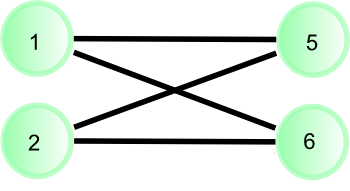
\includegraphics[scale=0.25]{./figuras/constructivas/insercionGreedyRandom/dibujo0.png} }
    \label{fig:posta}
    \subfigure[]{
    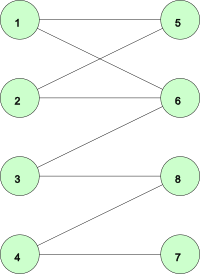
\includegraphics[scale=0.25]{./figuras/constructivas/insercionGreedyRandom/posta.png}}
    \caption{Dibujo de partida y dibujo �ptimo}       
\end{figure} 

A continuaci�n mostramos la ejecuci�n de la heur�stica. Los nodos marcados con
rojo son los que el algoritmo agrega en cada iteraci�n.

\begin{itemize}

\item Inserci�n con selecci�n aleatoria
\begin{figure}[H]
\centering
\setcounter{subfigure}{0}
\subfigure[]{
\includegraphics[scale=0.2]{./figuras/constructivas/insercionGreedyRandom/dibujo1.png}}
\subfigure[]{
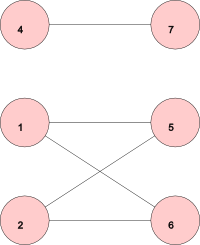
\includegraphics[scale=0.2]{./figuras/constructivas/insercionGreedyRandom/dibujo2.png}}
\subfigure[]{
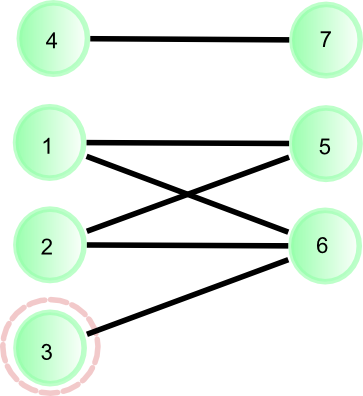
\includegraphics[scale=0.2]{./figuras/constructivas/insercionGreedyRandom/dibujo3.png}}
\subfigure[]{
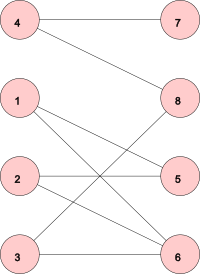
\includegraphics[scale=0.2]{./figuras/constructivas/insercionGreedyRandom/dibujo4.png}}
\end{figure}

\item Inserci�n con selecci�n por mayor grado

\begin{figure}[H]
\centering
\setcounter{subfigure}{0}
\subfigure[]{
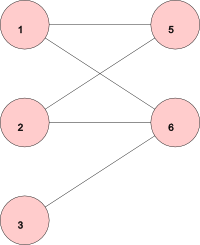
\includegraphics[scale=0.2]{./figuras/constructivas/insercionGreedyMayorGrado/dibujo1.png}}
\subfigure[]{
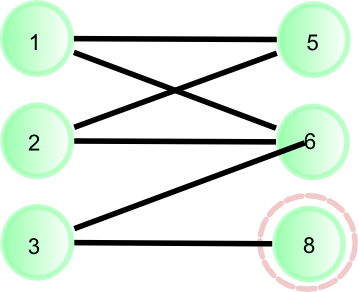
\includegraphics[scale=0.2]{./figuras/constructivas/insercionGreedyMayorGrado/dibujo2.png}}
\subfigure[]{
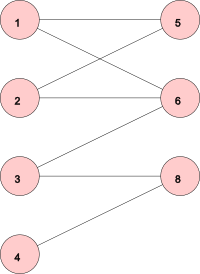
\includegraphics[scale=0.2]{./figuras/constructivas/insercionGreedyMayorGrado/dibujo3.png}}
\subfigure[]{
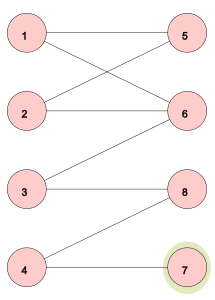
\includegraphics[scale=0.2]{./figuras/constructivas/insercionGreedyMayorGrado/dibujo4.png}}
\end{figure}

\item Inserci�n con selecci�n por menor grado
\begin{figure}[H]
\centering
\setcounter{subfigure}{0}
\subfigure[]{
\includegraphics[scale=0.2]{./figuras/constructivas/insercionGreedyMenorGrado/dibujo1.png}}
\subfigure[]{
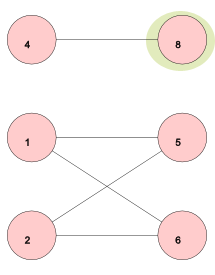
\includegraphics[scale=0.2]{./figuras/constructivas/insercionGreedyMenorGrado/dibujo2.png}}
\subfigure[]{
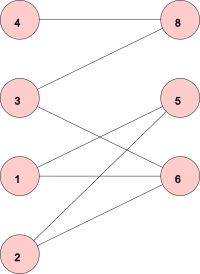
\includegraphics[scale=0.2]{./figuras/constructivas/insercionGreedyMenorGrado/dibujo3.png}}
\subfigure[]{
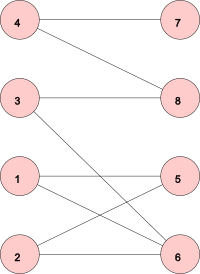
\includegraphics[scale=0.2]{./figuras/constructivas/insercionGreedyMenorGrado/dibujo4.png}}
\end{figure}
\end{itemize}


\subsubsection{Pseudoc�digo}

\begin{algorithm}[H]
\caption{Propone un dibujo mediante la inserci�n golosa de nodos}
\begin{algorithmic}[1]
\PARAMS{dibujo original a incrementar}
\STATE cruces $\leftarrow$ cruces del dibujo original
\WHILE{queden nodos por poner}
    \FOR{cada partici�n donde queden nodos m�viles por colocar}
        \STATE nodo $\leftarrow$ elegir uno entre los nodos m�viles
        \STATE sacar al nodo de entre los nodos a poner
        \STATE colocar al nodo en la ultima posici�n en su partici�n
        \STATE crucesNuevo $\leftarrow$ cruces + cruces que se producen al agregar el nodo atr�s de la particion
        \STATE mejorCruces $\leftarrow$ crucesNuevo
        \STATE mejorPos = ultima posici�n
        \WHILE{no se revisaron todas las posiciones dentro de la partici�n}
            \STATE mover al nodo a la proxima posici�n \COMMENT{``swapear'' al nodo con el que est� en la posici�n anterior}
            \STATE crucesPreSwap $\leftarrow$ cruces entre el nodo a insertar y el nodo anterior antes del \textit{swap}
            \STATE crucesPostSwap $\leftarrow$ cruces entre el nodo a insertar y el nodo anterior despu�s del \textit{swap}
            \STATE cruces $\leftarrow$ cruces - crucesPreSwap + crucesPostSwap
            \IF{ cruces $<$ mejorCruces}
            	\STATE mejorCruces $\leftarrow$ cruces
            	\STATE mejorPos $\leftarrow$ la posici�n que estoy verificando
            \ENDIF
        \ENDWHILE
    	\STATE poner al nodo en mejorPos
        \STATE cruces $\leftarrow$ mejorCruces
    \ENDFOR
\ENDWHILE
\end{algorithmic}
\end{algorithm} 


\subsection{Heuristica de inserci�n de ejes}

Una vez m�s partimos del dibujo original, pero en este caso procedemos agregando ejes:
tomamos un eje ``nuevo'' y insertamos sus extremos en el par de posiciones v�lidas
que minimiza el total de cruces en el dibujo obtenido. Entendemos por eje ``nuevo'' a
aquellos ejes que tienen al menos uno de sus extremos no fijado de antemano. En el caso
en que uno de los extremos del eje pertenezca al dibujo original (su posici�n relativa
a los otros nodos de ese dibujo es fija), este nodo podr�a de todos modos tener m�s de una posici�n
v�lida en el dibujo incrementado y por lo tanto se prueban todas las posiciones que
mantienen el orden relativo original. 

En cada iteraci�n, si uno de los nodos del eje
que se est� insertando ya fue fijado por una pasada anterior del algoritmo, se lo
extrae e inserta nuevamente. Si bien podr�a parecer que el algoritmo repite
c�lculos de forma redundante, esto no es necesariamente cierto puesto que se reinserta
un nodo cuya posici�n ya se hab�a establecido, el nuevo dibujo contiene m�s ejes
que el que se hab�a usado para tomar la decisi�n anterior, y por tanto la nueva
decisi�n ser� m�s ``informada'' que la primera desde un punto de vista heur�stico
(lo cual no implica que sea mejor). Este tipo de decisi�n permite que la inserci�n
de un nuevo eje pueda incluso disminuir la cantidad de cruces respecto del dibujo
anterior, cosa que era imposible en la heur�stica anterior (donde el n�mero de cruces
a lo sumo se mantiene igual en cada iteraci�n, pero nunca mejora).

Por estas diferencias podr�amos presuponer que esta heur�stica, al ser m�s
sofisticada que la anterior, podr�a obtener mejores resultados. Sin embargo,
el aumento de costo no es despreciable: para cada eje habr� que recorrer todos
los pares de posiciones posibles para sus dos extremos observando cuantos
ejes produce cada uno. Esto deber� ser tenido en cuenta cuando realicemos el
an�lisis experimental.

Si aplicamos la heur�stica para el grafo de \ref{fig:posta}, obtenemos lo siguiente:

\begin{figure}[H]
\centering
\setcounter{subfigure}{0}
\subfigure[]{
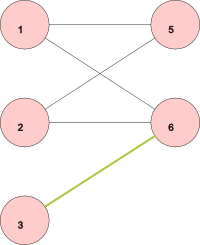
\includegraphics[scale=0.2]{./figuras/constructivas/insercionEjes/dibujo1.png}}
\subfigure[]{
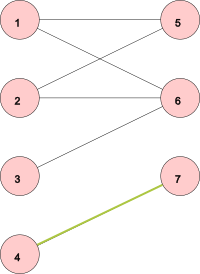
\includegraphics[scale=0.2]{./figuras/constructivas/insercionEjes/dibujo2.png}}
\subfigure[]{
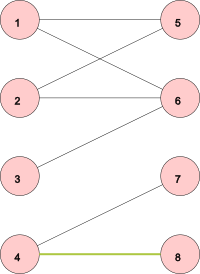
\includegraphics[scale=0.2]{./figuras/constructivas/insercionEjes/dibujo3.png}}
\subfigure[]{
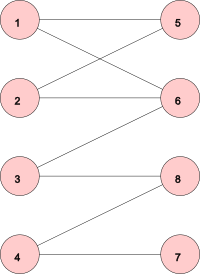
\includegraphics[scale=0.2]{./figuras/constructivas/insercionEjes/dibujo4.png}}
\end{figure}

Notemos como en el �ltimo paso, al agregar el eje $(3,8)$ se mueve al nodo 8 de 
la posici�n que le hab�a asignado antes, de modo de reducir la cantidad de cruces. 
Por otro lado observamos que si bien el algoritmo logr� la soluci�n �ptima, esto se
debi� a que cuando exist�a ambiguedad entre varias posiciones donde poner a los nodos
(debido a que todas ellas produc�an la misma cantidad de cruces), los puso abajo. Si 
hubiese elegido ponerlos arriba (opci�n v�lida, dado que genera la misma cantidad de 
cruces: 0) el resultado hubiera sido distinto.


\subsubsection{Pseudoc�digo}
\begin{algorithm}[H]
\caption{Propone un dibujo mediante la inserci�n golosa de ejes}
\begin{algorithmic}[1]
\STATE ejesPuestos $\leftarrow$ los ejes del dibujo original
\STATE puesto$[v_i]$ $\leftarrow$ �$v_i$ estaba en el dibujo original?
\FOR{cada eje $(x,y)$ a agregar}
    \IF{ya puse a $x$}
       \STATE sacarlo
    \ELSE
       \STATE puesto$[x]$ = True
    \ENDIF
    \IF{ya puse a $y$}
       \STATE sacarlo
    \ELSE
       \STATE puesto$[y]$ = True
    \ENDIF
    \STATE agregar el eje a ejesPuestos 
    \STATE agregar $x$ a la lista de adyacencia de $y$
    \STATE agregar $y$ a la lista de adyacencia de $x$
    \STATE calcular los rangos en los cuales puedo mover $x$ y $y$ \COMMENT{si alguno estaba en el dibujo original, hay que respetar el orden relativo}
    \STATE insertar $x$ en su primer posici�n v�lida
    \STATE insertar $y$ en su primer posici�n v�lida
    \STATE mejoresCruces $\leftarrow$ los cruces por ponerlos en esta posici�n
    \STATE mejorPosici�n $\leftarrow$ posici�n actual
    \FOR{cada posici�n v�lida para $x$}
        \FOR{cada posici�n v�lida para $y$}
            \STATE contar los cruces por dejarlos en esa posici�n
            \IF{generan menos cruces que mejoresCruces}
               \STATE mejoresCruces $\leftarrow$ cruces por tenerlos en esta posici�n
               \STATE mejorPosicion $\leftarrow$ posici�n actual
            \ENDIF
            \STATE mover $y$ a su proxima posici�n
        \ENDFOR
        \STATE mover $x$ a su pr�xima posici�n v�lida
        \STATE mover $y$ a su primer posici�n v�lida
    \ENDFOR
    \STATE mover $x$ y a $y$ a la mejorPosicion
\ENDFOR
\end{algorithmic}
\end{algorithm} 


\subsection{Heur�stica de inserci�n de nodos por mediana}

La idea general de esta heur�stica es buscar que ning�n nodo este demasiado 
``lejos'' de sus adyacentes. Como criterio heur�stico para lograr esto,
utilizamos como posici�n de un nodo la mediana de las posiciones de sus
adyacentes.

El procedimiento es el siguiente: en un principio se comienza con solamente 
los nodos que ya estaban en el dibujo original acompa�ados de sus ejes.
Tomamos entonces al nodo de mayor grado (con respecto a los nodos que ya est�n
puestos, an�logamente a la primera heur�stica), calculamos la mediana de las 
posiciones de sus adyacentes y una vez que la obtenemos, probamos insertar 
al nodo en la posici�n correspondiente a la mediana obtenida, o en las posiciones
inmediata anterior o posterior a �sta, eligiendo de las tres a la que genere menos
cruces en el dibujo. En el caso en que la mediana no sea un �ndice v�lido (porque 
una partici�n tiene menos nodos que la otra, y el valor de la mediana se calcula a 
partir de la posici�n de los nodos de la m�s grande, y por tanto la mediana podr�a
ser mayor que el tama�o de la partici�n m�s chica) la truncamos. Repetimos el 
procedimiento iterativamente hasta que est�n puestos todos los nodos.

\begin{figure}[H]
\centering
\setcounter{subfigure}{0}
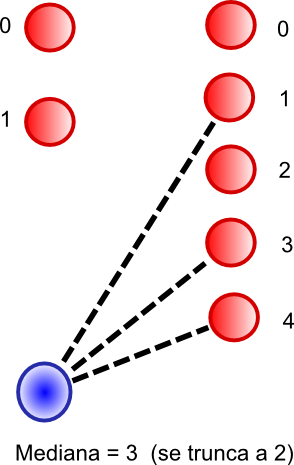
\includegraphics[scale=0.25]{./figuras/constructivas/medianaTruncada.png}
\caption{ejemplo de inserci�n por mediana con truncamiento}
\end{figure}

Al igual que en la heur�stica de inserci�n de nodos, si hab�a ejes a agregar 
entre los nodos que ya estaban, estos se agregan al inicio del algoritmo para 
dar m�s informaci�n a las posteriores inserciones.

Si aplicamos la heur�stica a \ref{fig:posta} lo que se obtiene es, en este caso,
la misma secuencia que en la heur�stica de inserci�n \textit{greedy} de nodos. Esto
se debe a que siempre se agregan nodos que tienen un �nico adyacente, y �ste est� 
ubicado al final de la partici�n vecina.

Esta heur�stica utiliza un criterio \textit{greedy} que podr�amos calificar de
indirecto: las otras heur�sticas son \textit{greedy} en el sentido que minimizan
el n�mero de cruces de cada inserci�n (minimizan localmente el mismo criterio que
debe minimizarse globalmente), mientras que la de la mediana utiliza como
criterio local la distancia a la que queda cada nodo de sus adyacentes. Es una 
heur�stica similar a la del baricentro, que en el caso del problema de dibujo de 
grafos bipartitos sin la caracter�stica de ser incrementales se comporta de forma
muy favorable. %TODO citar paper :p

Como mejora adicional, Luego de ubicar a todos los nodos, se hace una pasada 
en cada partici�n intercambiando nodos en posiciones consecutivas si esta permutaci�n
disminuye el n�mero total de cruces del dibujo. Esto se hace con el objetivo de paliar
los problemas originados por el truncamiento de los valores de las medianas descripto
anteriormente.


\subsubsection{Pseudoc�digo}

\begin{algorithm}[H]
\caption{Propone un dibujo mediante inserci�n por la mediana de los adyacentes}
\begin{algorithmic}[1]
\WHILE{queden nodos sin poner}
    \STATE elegir un nodo de grado m�ximo con respecto a los que ya est�n puestos
    \STATE calcular la mediana de las posiciones de sus adyacentes
    \IF{mediana $>$ tama�o actual de la partici�n}
        \STATE mediana $\leftarrow$ tama�o de la partici�n
    \ENDIF
    \FOR{ cada i = mediana-1, mediana, mediana+1}
        \IF{es una posici�n v�lida}
            \STATE contar los cruces por ponerlo en esa posici�n
            \IF{lo insert� por primera vez o me genera menos cruces que la mejorPosicion}
                \STATE mejorPosicion $\leftarrow$ posicionActual
            \ENDIF
        \ENDIF
    \ENDFOR
    \STATE poner al nodo en mejorPosicion
\ENDWHILE
\end{algorithmic}
\end{algorithm} 








\section{Comparaci�n de las heur�sticas constructivas}

A fin de decidir cual o cuales de estas heur�sticas se comporta mejor, y al
igual que con el algoritmo exacto, decidimos hacer primero una implementaci�n en 
Python por las facilidades que da el lenguaje en cuanto a velocidad de desarrollo. 
Utilizando estas implementaciones, aplicamos las heur�sticas a numerosos casos de prueba
y comparamos los resultados, teniendo en cuenta no solo la calidad de los resultados
obtenidos sino tambi�n el costo temporal.

A priori lo que esperamos es que la heur�stica de inserci�n de ejes de mejores 
resultados por el hecho de que reinserta nodos, lo cual le da varias oportunidades para 
fijar la posici�n de un nudo dado, por lo cual podr�a corregir errores cometidos por 
insertar cuando todav�a hab�a pocos nodos en el dibujo.

Sin embargo, es de esperarse que este m�todo sea considerablemente m�s lento que los dem�s:
en primer lugar, porque itera tantas veces como ejes se agreguen, lo cual podr�a ser $O(n^2)$ 
siendo $n$ la cantidad de nodos, y en segundo lugar porque cada una de estas iteraciones 
requiere de $O(n^2)$ conteos de cruces. Si a esto le sumamos el costo de contar los 
cruces vemos que el costo de esta heur�stica es bastante elevado.

Respecto de la heur�stica de la mediana, resulta dif�cil prever como se comportar�
el algoritmo. Si bien es de esperarse que tenga un costo temporal reducido (ya que solo
``prueba'' tres posiciones para cada nodo y por lo tanto realiza pocos conteos de cruces),
su performance no es f�cil de predecir.

Finalmente, respecto a la inserci�n \textit{greedy} de los nodos, creemos que su costo 
ser� menor que el de la inserci�n de ejes, pero sus resultados podr�an no ser tan buenos
en raz�n de su simpleza inherente.

Ejecutamos los siguientes tests:
\begin{enumerate}
\item Comparaci�n de Heuristicas de inserci�n \textit{greedy} de nodos:
    Primero comparamos a las diferentes formas de elegir al nodo candidato, para 
    observar si alguna de las formas de hacerlo se desempe�a mejor.

\item Comparaci�n entre heur�sticas:
    \begin{enumerate}
    \item $n$ nodos en cada partici�n, $n$ creciente, $\frac{n^2}{2}$ ejes, 60\% de nodos nuevos
    \item $n$ nodos en cada partici�n, $n$ creciente, $\frac{n^2}{2}$ ejes, 40\% de nodos nuevos
    \item $n$ nodos en cada partici�n, $n$ creciente, $3n$ ejes, 60\% de nodos nuevos
    \item $n$ nodos en cada partici�n, $n$ creciente, $3n$ ejes, 40\% de nodos nuevos
    \item $n = 30$, cantidad de ejes creciente, 40\% de nodos nuevos
    \end{enumerate}
\end{enumerate}

En cada uno de ellos se midi� sobre grafos aleatorios de los tama�os mencionados la cantidad 
de cruces lograda y el tiempo empleado para lograr el dibujo.

Si bien los tiempos de ejecuci�n en un lenguaje interpretado como Python, son por lo 
general bastante mayores que los tiempos de ejecuci�n en C++, consideramos que son 
igualmente v�lidos como herramienta de comparaci�n para observar una tendencia general 
en el comportamiento de las heur�sticas. Por otro lado, dado que implementar en este 
lenguaje nos resulta mucho m�s sencillo, consideramos que vale la pena probar a tres 
heur�sticas experimentalmente en lugar de proponer una �nica para implementar en C++.

\subsection{Criterios de selecci�n de nodos para la heur�stica de inserci�n de nodos}
Las pruebas que realizamos consistieron en aplicar la heur�stica de inserci�n de nodos 
a grafos aleatorios variando la cantidad de nodos en cada partici�n.

En la primer experiencia utilizamos grafos con $m=2*n$ y un $40\%$ de nodos fijos (en 
adelante $n$ es la cantidad de nodos de cada partici�n). En la segunda experiencia, 
la cantidad de ejes fue $m=\frac{n^2}{2}$ y el porcentaje de nodos fijos fue tambi�n del $40\%$.

\begin{figure}[H]
\centering
\setcounter{subfigure}{0}
\subfigure[]{
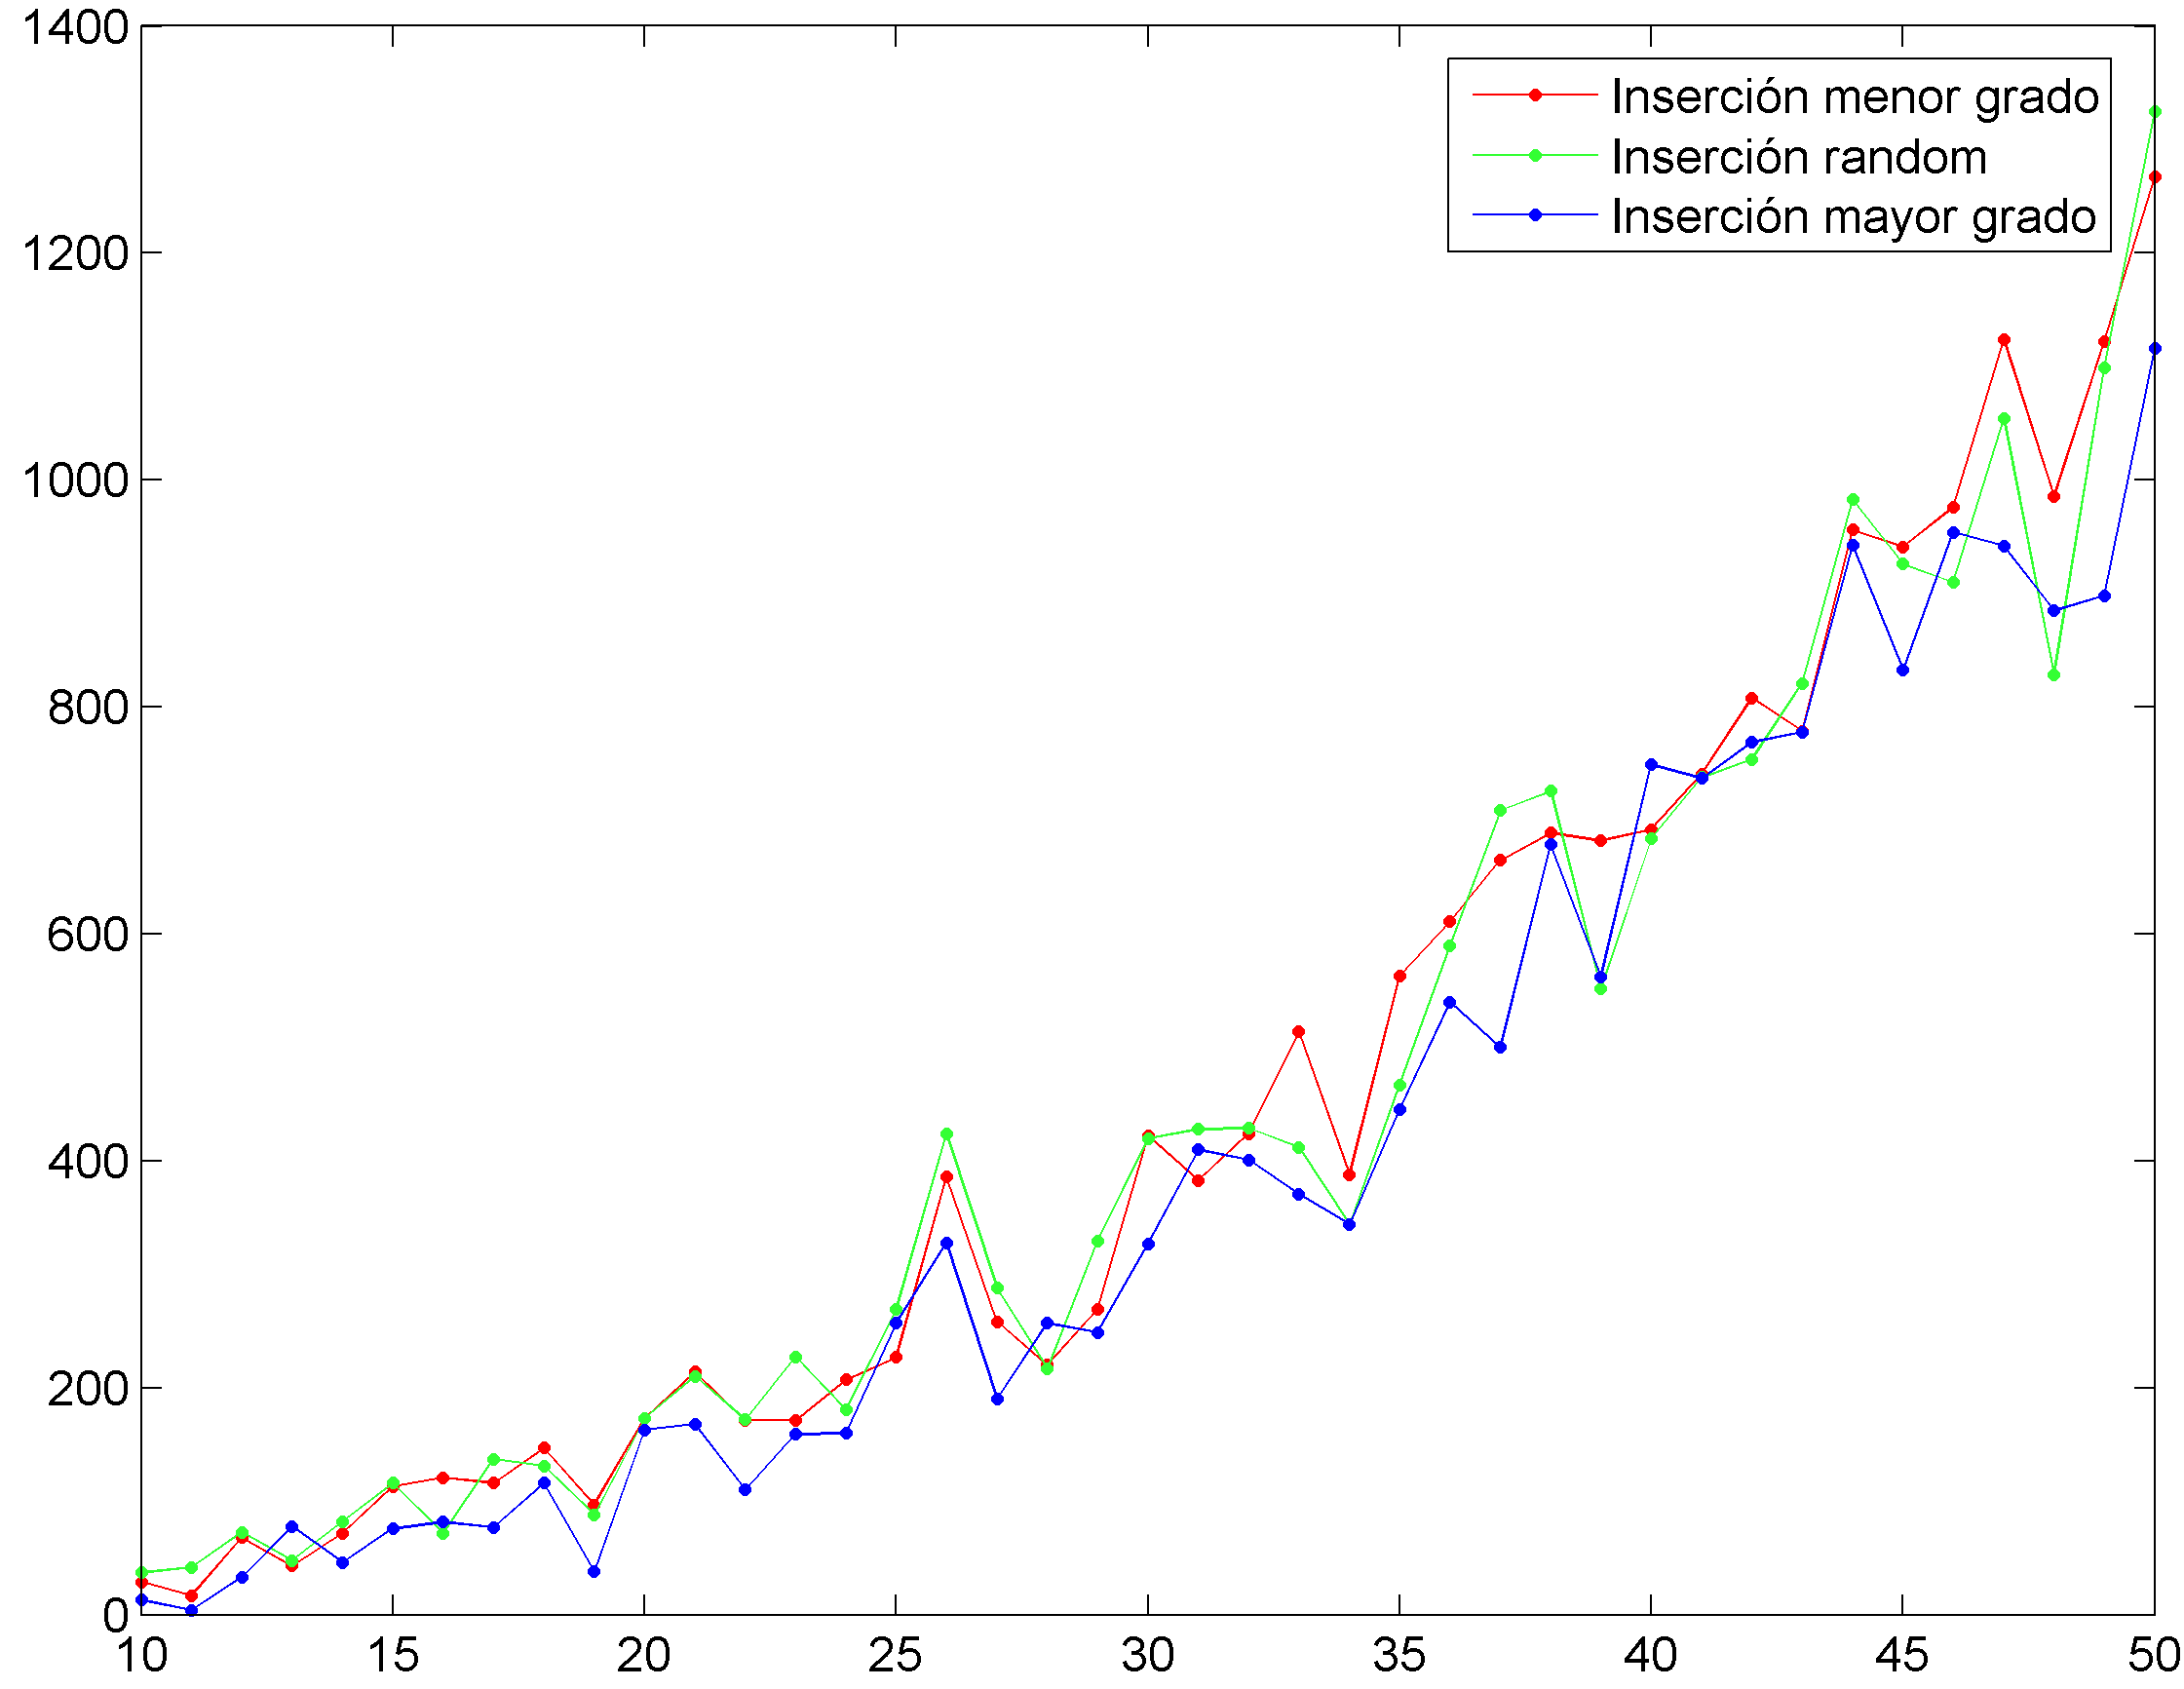
\includegraphics[scale=0.6]{./graficos/comparacionInsercionNodos/exp2.png}}
\subfigure[]{
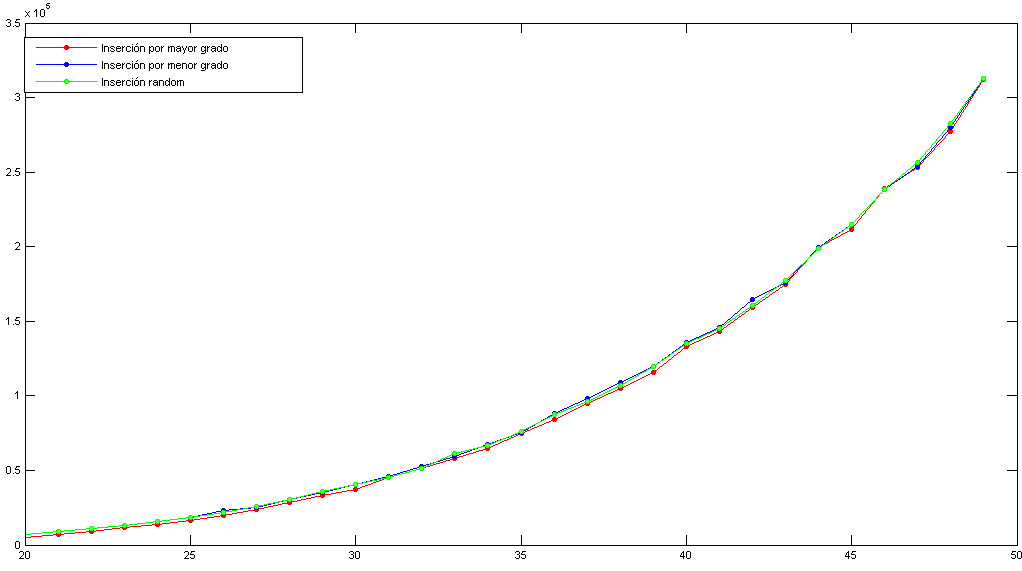
\includegraphics[scale=0.6]{./graficos/comparacionInsercionNodos/exp1.png}} 
\end{figure}

Observamos en estas experiencias que la cantidad de cruces encontrada por los 
tres m�todos es relativamente similar. Sin embargo el criterio de mayor grado 
parecer�a comportarse ligeramente mejor que los otros dos. Para nosotros tiene 
sentido que esto sea as�, ya que si se utiliza el nodo de mayor grado con respecto
a lo que ya est� puesto, ese nodo tiene m�s informaci�n (mas adyacentes puestos) 
por lo que ser�a razonable que pueda ubicarse mejor. Est� claro que podr�a fallar, 
sin embargo a partir de esta idea, m�s lo que se observa en las pruebas, decidimos 
utilizar al nodo de mayor grado para la heur�stica de inserci�n de nodos.

\subsection{Comparaci�n de heur�sticas constructivas}

\begin{figure}[H]
\centering
\setcounter{subfigure}{0}
\subfigure[Cruces producidos en funci�n de $n$]{
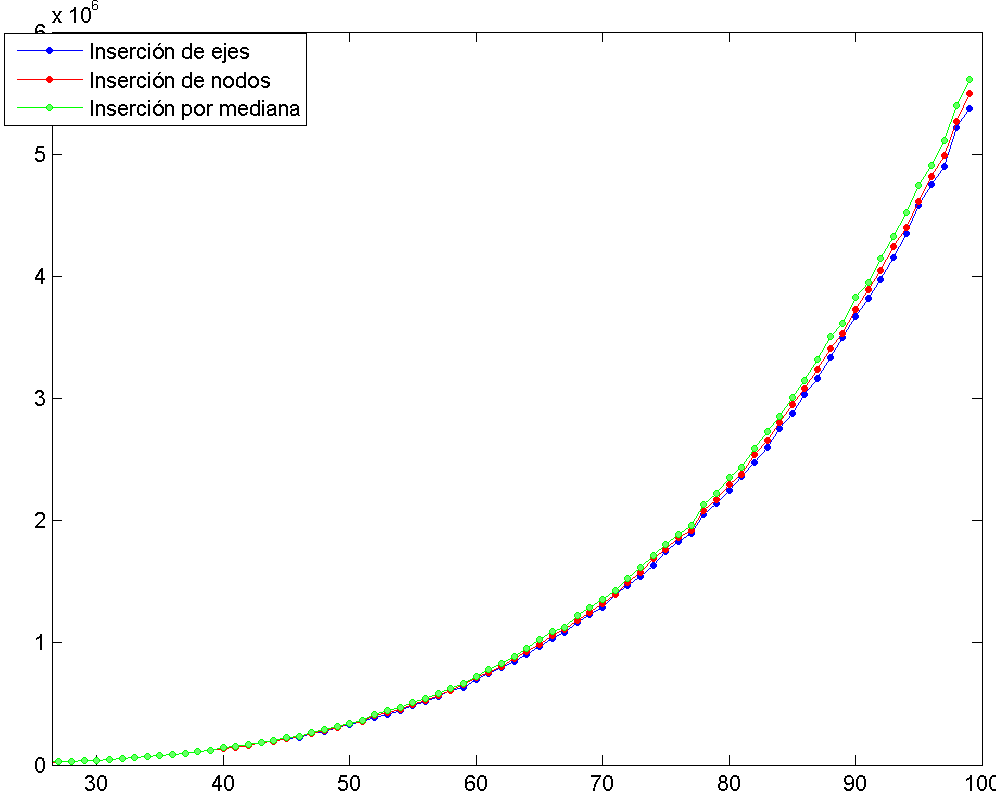
\includegraphics[scale=0.61]{./graficos/comparacionConstructivas/cruces1.png}}
\setcounter{subfigure}{1}
\subfigure[Tiempo en segundos en funci�n de $n$]{
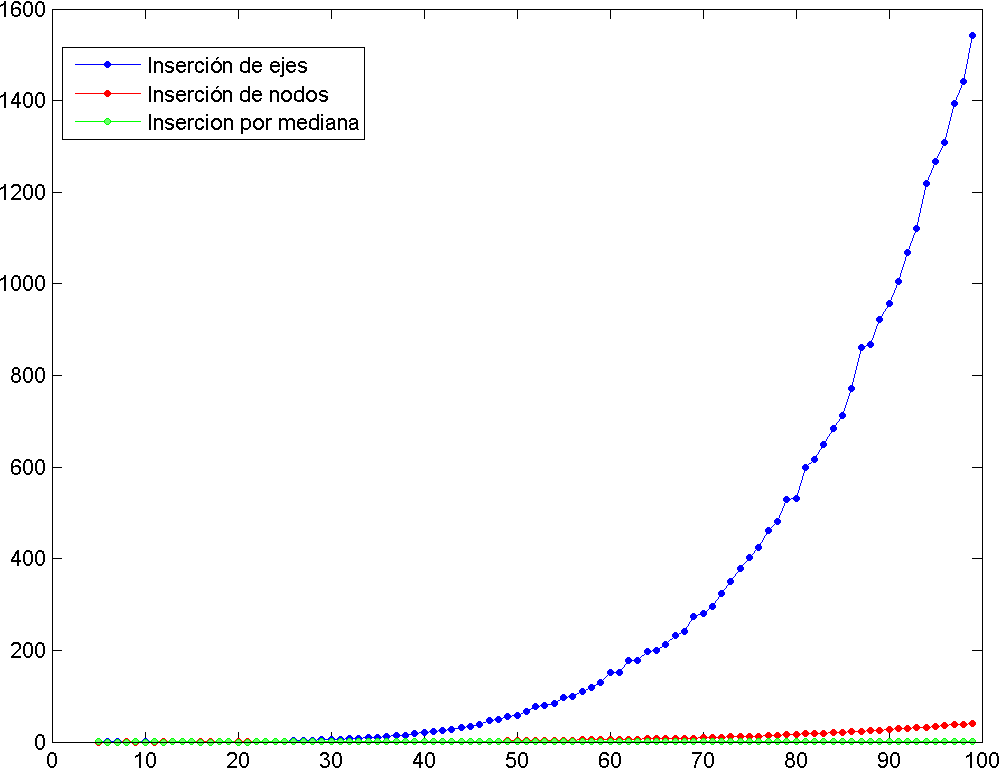
\includegraphics[scale=0.61]{./graficos/comparacionConstructivas/tiempos1.png} }
\caption{$n$ nodos en cada partici�n, $n$ creciente, $\frac{n^2}{2}$ ejes, 60\% de nodos nuevos}
\end{figure}

\begin{figure}[H]
\centering
\setcounter{subfigure}{0}
\subfigure[Cruces producidos en funci�n de $n$]{
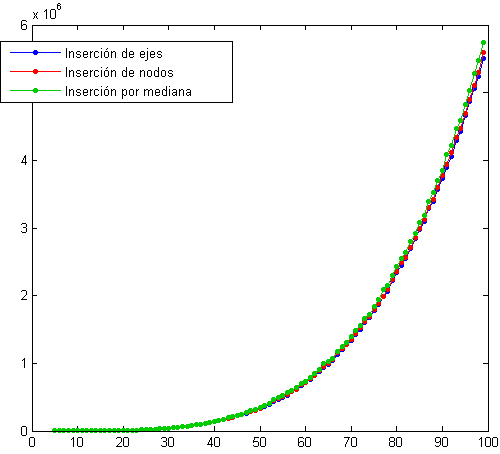
\includegraphics[scale=0.61]{./graficos/comparacionConstructivas/cruces2.png}}
\setcounter{subfigure}{1}
\subfigure[Tiempo en segundos en funci�n de $n$]{
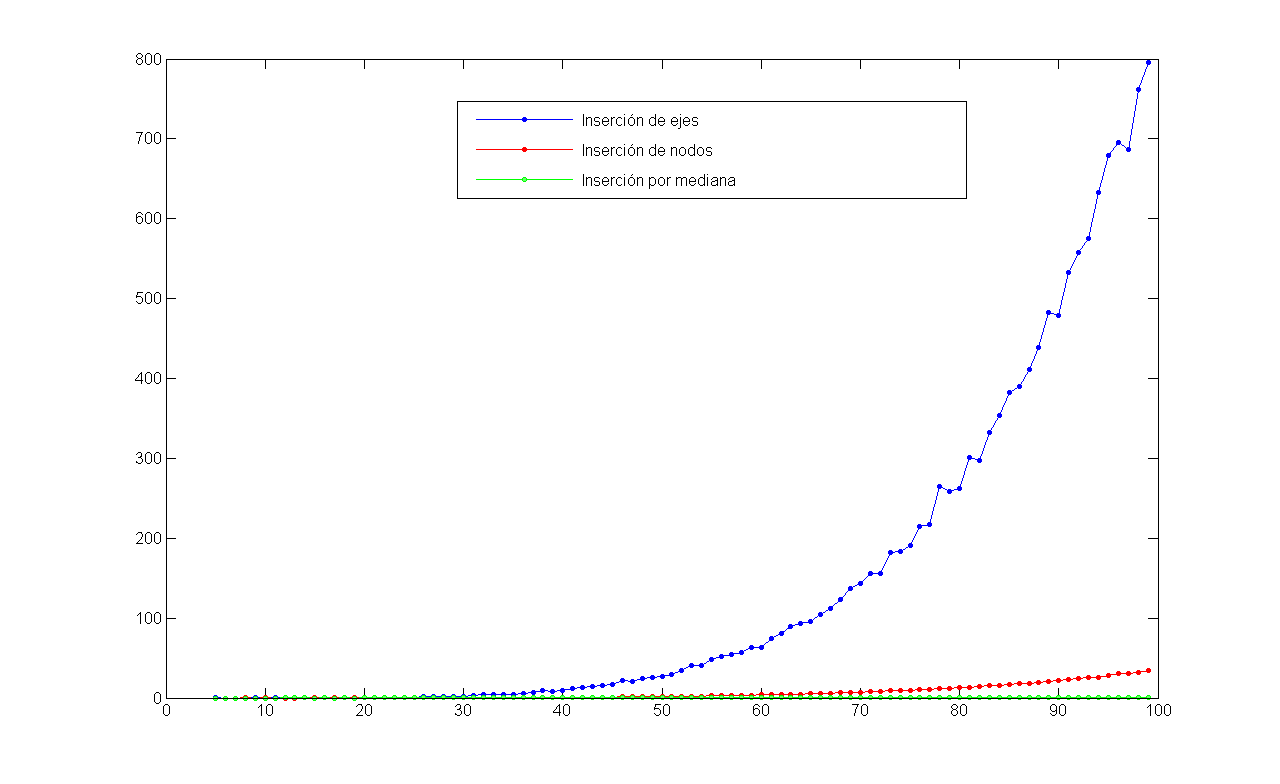
\includegraphics[scale=0.61]{./graficos/comparacionConstructivas/tiempos2.png} }
\caption{$n$ nodos en cada partici�n, $n$ creciente, $\frac{n^2}{2}$ ejes, 40\% de nodos nuevos}
\end{figure}

\begin{figure}[H]
\centering
\setcounter{subfigure}{0}
\subfigure[Cruces producidos en funci�n de $n$]{
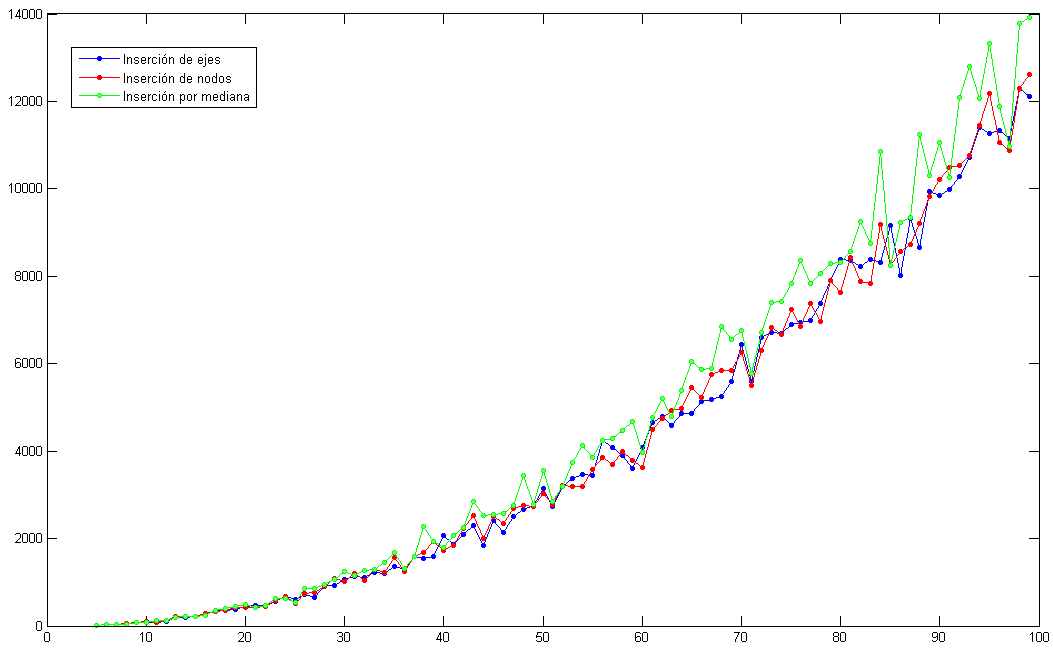
\includegraphics[scale=0.61]{./graficos/comparacionConstructivas/cruces3.png}}
\setcounter{subfigure}{1}
\subfigure[Tiempo en segundos en funci�n de $n$]{
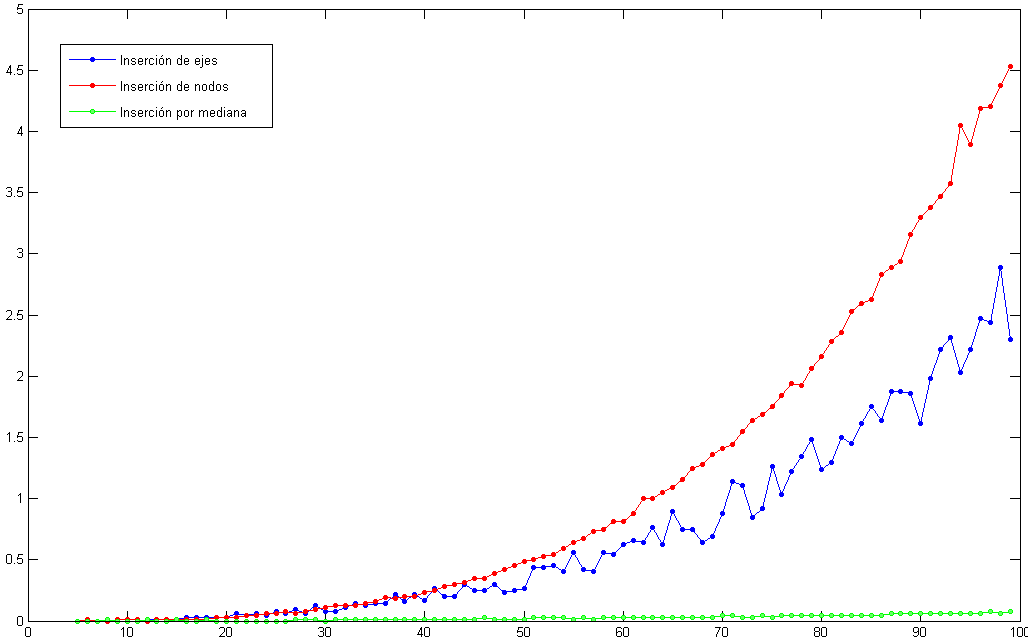
\includegraphics[scale=0.69]{./graficos/comparacionConstructivas/tiempos3.png} }
\caption{$n$ nodos en cada partici�n, $n$ creciente, $3n$ ejes, 60\% de nodos nuevos}
\end{figure}

\begin{figure}[H]
\centering
\setcounter{subfigure}{0}
\subfigure[Cruces producidos en funci�n de $n$]{
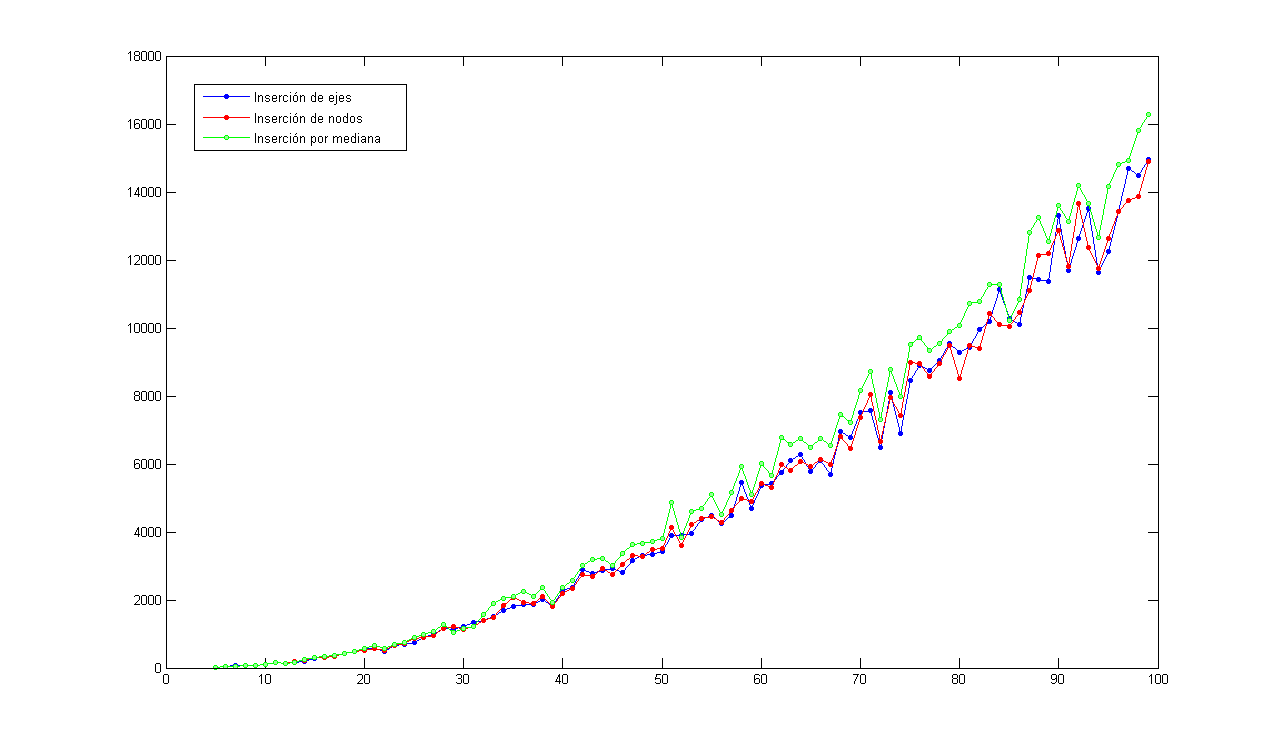
\includegraphics[scale=0.61]{./graficos/comparacionConstructivas/cruces4.png}}
\setcounter{subfigure}{1}
\subfigure[Tiempo en segundos en funci�n de $n$]{
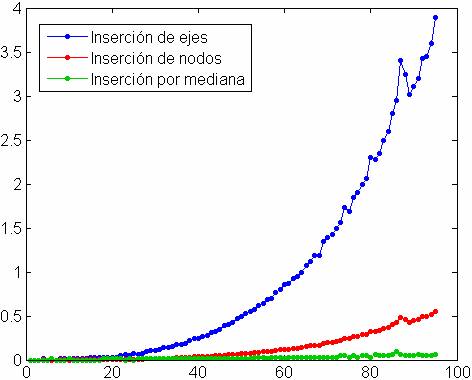
\includegraphics[scale=0.67]{./graficos/comparacionConstructivas/tiempos4.png} }
\caption{$n$ nodos en cada partici�n, $n$ creciente, $3n$ ejes, 40\% de nodos nuevos}
\end{figure}

\begin{figure}[H]
\centering
\subfigure[Cruces producidos en funci�n de $m$]{
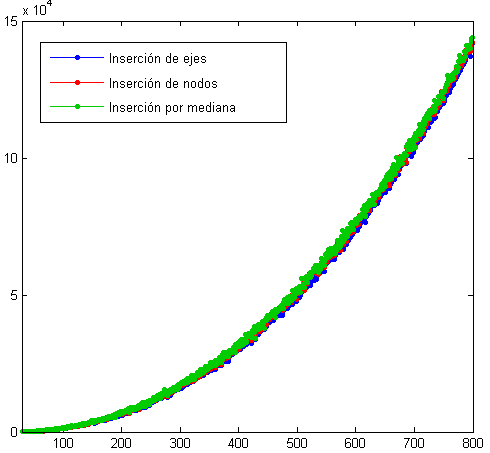
\includegraphics[scale=0.61]{./graficos/comparacionConstructivas/cruces5.png}}
\subfigure[Tiempo en segundos en funci�n de $m$]{
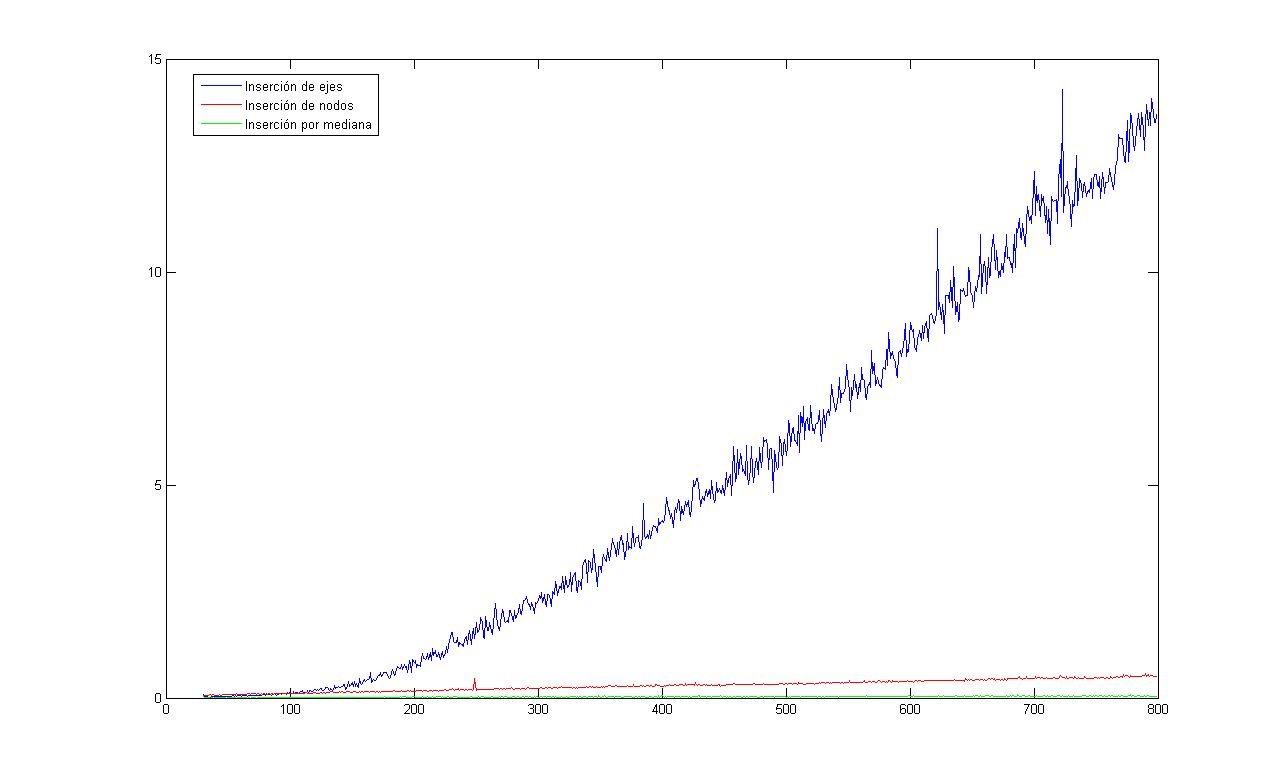
\includegraphics[scale=0.61]{./graficos/comparacionConstructivas/tiempos5.png} }
\caption{ $n = 30$, $m$ creciente, 40\% de nodos nuevos}
\setcounter{subfigure}{0}
\end{figure}


\section{An�lisis de los resultados}

Al observar los gr�ficos de las experiencias lo primero que salta a la vista es 
que el tiempo de ejecuci�n de la heur'istica de inserci�n de ejes es mucho m�s 
grande que el de las dem�s. Esta situaci�n, que se hace m�s notoria en grafos densos, 
hace que su uso no sea recomendable, m�s a�n si tenemos en cuenta como muestran las dem�s
experiencias que los resultados que obtiene no son significativamente mejores que los de
las otras. En la experiencia 5 vemos como para un grafo con 30 nodos y 799 ejes la diferencia entre 
la inserci�n de nodos y la inserci�n de ejes de 442 cruces a favor de la inserci�on de ejes 
(142131 contra 141689), lo cual es s�lo un 0.3\%, pero los tiempos fueron de 0.5160 y 13.6870
segundos respectivamente, lo cual es aproximadamente 26 veces m�s. En funci�n de esta
ineficiencia temporal, si bien los resultados que ofrece son buenos, decidimos descartar
la heur�stica de inserci�n de ejes.

Por otro lado, la heur�stica de la mediana se muestra como la m�s r�pida, como hab�amos
estimado previamente. Sin embargo en cuanto a la cantidad de cruces suele dar peores 
resultados que las otras dos. Es por esto, que decimos entonces descartar la heur�stica
de la mediana por obtener resultados de peor calidad sin un ahorro sustancial de tiempo
de ejecuci�n.

Finalmente elegimos implementar en C++ la heur�stica de inserci�n de nodos, ya que 
consideramos que de las tres alternativas planteadas obtiene un buen compromiso entre
calidad de los resultados y tiempos cortos de ejecuci�n. 

\section{Detalles de implementaci�n}

La implementaci�n al igual que en el caso del algoritmo exacto, utiliza diversos
contenedores de la STL. Si se observa el c�digo en C++ hay algunas modificaciones
respecto del algoritmo presentado hasta el momento que responden a los cambios
realizados para agregar factores aleatorios a las soluciones propuestas por la 
heur�stica. Estas modificaciones son necesarias para la implementaci�n de GRASP
y son detalladas en \ref{modificaciones_constructiva}. 

Como particularidad de implementaci�n se puede mencionar el uso de \verb0std :: sort0
para ordenar la secuencia de nodos por insertar seg�n su grado de adyacencias
(si solo se debe tomar el m�ximo esto es ineficiente, pero en el contexto del GRASP
donde deben tomarse los $k$ primeros elementos es lo m�s conveniente). Para este
fin se utiliza un objeto adaptador que es el responsable de las comparaciones
entre elementos seg�n su grado.

%FIXME: unificar notacion
%FIXME: revisar si el orden esta bien, ademas si esta bien expresarlo asi. Por ej. se suprime un movil*log(movil) que tal vez este bueno dejar
\section{C�lculo de complejidad}
\label{complejidadDeLaConstructiva}
Antes de comenzar, realizamos una limpieza del grafo, para no considerar a los nodos que tienen
grado nulo. Como comentamos en el apartado \ref{sacoNulos}, esto tiene un costo $O(V_1+V_2+m)$ donde 
$V_i$ es la cantidad de nodos de partici�n $i$ sin filtrar y $m$ la cantidad de ejes. Este costo se 
deber� sumar a la complejidad total.

La heur'istica de inserci'on de nodos comienza asignando variables y atributos 'utiles para la reutilizaci'on 
de c'alculos. Inicializamos dos listas de nodos fijos y dos de nodos a agregar (un par para cada partici'on), 
y los diccionarios de adyacencias parcial, grado parcial, posiciones y nodos m�viles. Todo esto tiene un costo 
de $O(v_{max} + m)$. Adem'as, en esta parte inicializamos la variable $cruces$, contando los cruces del 
dibujo original (fijo) sin agregar ning'un nodo, lo que nos cuesta $O(m*log(fijos_{max})+fijos_{max}))$.
Finalmente la parte de inicializaci'on nos cuesta $O(n + m + m*log(fijos_{max})+fijos_{max})$, con $m$ su 
cantidad de ejes, y $fijos_{max}$ la cantidad de nodos fijos de la partici'on que tiene m'as nodos fijos.

Veamos ahora cuanto nos cuesta elegir un nodo entre los nodos a agregar. Primero ordenamos de forma creciente
(con sort de STL) los nodos a agregar por su grado parcial (considerando solamente los ejes que van del nodo 
hacia un nodo fijo o del nodo hacia un nodo que ya fue agregado al dibujo en iteraciones previas).
Este ordenamiento tiene complejidad $O(cantMovilesPi*log(cantMovilesPi))$. Si bien para tomar el m�ximo
valor no es necesario ordenar, las extensiones futuras vinculadas con la aleatorizaci�n del algoritmo
si requieren de disponer de la secuencia ordenada. Por esta raz�n, consideramos este costo como una cota de peor
caso de todas las variantes del algoritmo. 

Luego de ordenarlos, tomamos el primero de la secuencia. Luego estos pasos tienen un costo 
$O(cantMovilesPi*log(cantMovilesPi))$, siendo $Pi$ la partici'on sobre la cual estamos agregando el nodo.
%iteramos la secuencia hasta que el grado maximo sea mayor al grado del nodo en la posici�n que estamos mirando y de estos nodos nos quedamos con uno, esto nos cuesta $O(cantMovilesPi)$. Luego estos pasos tienen un costo $O(cantMovilesPi + cantMovilesPi*log(cantMovilesPi))$, siendo Pi la partici'on sobre la cual estamos agregando el nodo.

Ahora buscamos una de las mejores posiciones en la partici'on para insertar este nodo. Primero 
actualizamos la lista de adyacencias parciales para incorporar las adyacencias del nodo que voy a agregar 
(esto es necesario pues las funciones de conteo de cruces se usan dentro del subgrafo fijo y por tanto para 
que tengan en cuenta al nodo a agregar, es necesario completarlas con sus ejes) y luego insertamos el nodo 
al final de la partici'on.

Actualizar la lista de adyacencias parcial tiene un costo $O(m_a)$, con $m_a$ los ejes del nodo a agregar. 
Sin embargo, una vez que se agregan todos los nodos, en el peor de los casos se agregan todos los ejes tambi�n, 
por lo que esto tiene un costo $O(m)$. Luego contamos los cruces por agregar atr�s, lo cual tiene un costo 
$O(v_{max}+m)$. Ahora \textit{swapeamos} el nodo con su nodo anterior de la partici�n y recalculamos los 
cruces hasta que el nodo a agregar queda primero en la partici�n. Aqu'i podemos utilizar lo mostrado en 
el apartado que explica el conteo de cruces, y lo hacemos con costo $O(min(max(vi,m_a,m_b),m_a*m_b))$. Repetir
este proceso por cada posici'on en la partici'on que estamos agregando, tiene un costo de 
$O(cantModosParticion * min(max(vi,m_a,m_b),m_a*m_b))$. Adem�s, $max(v_i, m_a, m_b) \leq v_{max}$, puesto que $m_a$ 
y $m_b$ son a lo sumo tan grandes como la partici�n mas grande (en el caso en el que los nodos est�n relacionados con 
todos los de la partici�n de enfrente) y tambi�n vale $min(max(vi,m_a,m_b),m_a*m_b) \leq max(vi,m_a,m_b)$. De esto
resulta que la complejidad de este ciclo nos queda $O(v_{max}^2)$.

Finalmente, insertamos el nodo y actualizamos los grados parciales y el vector de posiciones, con un costo de $O(m + v_{max})$.

Dado que este procedimiento lo hacemos para todos los nodos a agregar, la complejidad resultante es: 

$$O(cantMoviles*(\underbrace{m + v_{max}}_{a} + \underbrace{v_{max}^2}_{b} + \underbrace{Moviles + MovilesP1*log(MovilesP1) + MovilesP2*log(MovilesP2))}_{c} + \underbrace{m*log(p_{max})+p_{max}}_{d})  (*)$$ 

\begin{itemize}
\item $a$ es por agregar al nodo atr�s de la partici�n
\item $b$ es por moverlo por toda la partici�n mediante \textit{swaps}
\item $c$ es por obtener cada vez uno de grado m�ximo
\item $d$ es por obtener por primera vez los cruces
\end{itemize}

Pero $* \subseteq O(Moviles*v_{max}^2 + m*log(fijos_{max})+fijos_{max})$, siendo Moviles 
la cantidad total de nodos a agregar, $v_{max}$ la cantidad de nodos de la partici'on m�s 
grande del dibujo resultante, $m$ la cantidad de ejes del dibujo resultante y $p_{max}$ la 
cantidad de nodos fijos de la partici'on que m'as nodos fijos tiene.

Esto es as� porque:

$O(m+v_{max}) \subseteq O(Moviles*v_{max}^2)$ dado que $m \leq v_{max}*v_{max}$ 

$O(MovilesPi + MovilesPi*log(MovilesPi)) \subseteq O(MovilesPi*log(MovilesPi))$, y como 
$MovilesPi*log(MovilesPi) \leq v_{max}*log(v_{max}) \leq v_{max}*v_{max}$, vale 
que $O(MovilesPi + MovilesPi*log(MovilesPi)) \subseteq  O(v_{max}^2)$

Finalmente, a esta complejidad obtenida debemos agregarle el costo de la ``limpieza'' del 
grafo. Por lo tanto, la complejidad total es:
$$O(Moviles*v_{max}^2 + m*log(fijos_{max})+fijos_{max}+ V_{1}+V_2+m)$$

El tama�o de la entrada $t$, lo podemos definir de la siguiente manera:

$$ t = log(P_1)+ \sum_{i=1}^{P_1}{log((p_1)_i)}+ log(P_2)+ \sum_{i=1}^{P_2}{log((p_2)_i)} + log(m_p) + \sum_{i=1}^{m_p}{log((e_i)_0) + log((e_i)_1)} $$
 $$+log(IV_1) + \sum_{i=1}^{IV_1}{log((iv_1)_i)} + log(IV_2) + \sum_{i=1}^{IV_2}{log((iv_2)_i)} + log(m_{iv})+ \sum_{i=1}^{m_{iv}}{log((e'_i)_0) + log((e'_i)_1)} $$ 

donde $P_i$ es la cantidad de nodos originales de la primera partici�n, $m_p$ es la cantidad 
de ejes originales, $IV_i$ es la cantidad de nodos que se agregan a la partici�n $i$ y $m_iv$ es 
la cantidad de ejes que se agregan.

Luego vale que:
$$t \geq log(P_1)+ v_1+ log(P_2)+V_2 + log(m_p) +m +log(IV_1) + log(IV_2) + log(m_{iv})$$
 
A partir de esto, vemos que:
$$ t \geq V_i \geq v_i$$
$$ t \geq V_{max} \geq v_{max}$$
$$ t \geq Moviles$$
$$ t \geq fijos_{max}$$
$$ t \geq m $$

Y por lo tanto resulta que el orden de toda la heur�stica es:
$$O(Moviles*v_{max}^2 + m*log(fijos_{max})+fijos_{max}+ V_{1}+V_2+m) \subseteq O(t^3 + t*log(t)+t) \subseteq O(t^3)$$ 

\section{An�lisis de la heur�stica}
\subsection{Casos patol�gicos}
\label{mal-caso} 

Para ver qu� tan malo podr�a ser el comportamiento de nuestra heur�stica, 
intentamos buscar casos donde el resultado que proponga el algoritmo diste 
arbitrariamente de la soluci�n �ptima.

Un caso donde la heur�stica se equivoca es el siguiente:

\begin{figure}[H]
\centering
\setcounter{subfigure}{0}
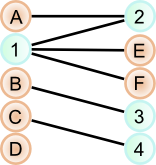
\includegraphics[scale=0.25]{./figuras/constructivas/malCasoConstructivo.png}
\caption{Caso patol�gico para la heur�stica constructiva}
\end{figure}

En este ejemplo los nodos numerados son los nodos que se agregan, mientras que 
los que tienen letras son los del dibujo original.

Veamos qu� hace la heur�stica constructiva frente a este caso:
\begin{figure}[H]
\centering
\setcounter{subfigure}{0}
\subfigure[Partimos del dibujo original]{

\includegraphics[scale=0.2]{./figuras/constructivas/malCons0.png}}\hspace{0.1in}
\subfigure[El 1 tiene mayor grado hacia lo que ya est�. Como sirve cualquier posici�n, lo insertamos en la primera que probamos (recordar que vamos desde atr�s hacia adelante)]{
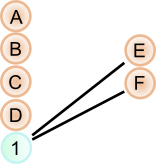
\includegraphics[scale=0.2]{./figuras/constructivas/malCons1.png} }\hspace{0.1in}
\subfigure[La mejor posici�n para el nodo 2 es arriba de todo ya que no genera cruces]{
\includegraphics[scale=0.2]{./figuras/constructivas/malCons2.png}}\hspace{0.1in}
\subfigure[El nodo 3 est� obligado a colocarse en una posici�n que genera un cruce]{
\includegraphics[scale=0.2]{./figuras/constructivas/malCons3.png}}\hspace{0.1in}
\subfigure[Ocurre lo mismo para el nodo 4]{
\includegraphics[scale=0.2]{./figuras/constructivas/malCons4.png}}
\end{figure}

Como vemos, en este caso, frente a un grafo para el cual existe un dibujo sin ning�n
cruce, nuestra heur�stica obtiene un dibujo con 2 cruces. Ahora bien, si tuvi�ramos 
un nodo nuevo m�s que estuviera relacionado con $D$, el dibujo �ptimo seguir�a teniendo 0 cruces, 
y sin embargo nuestra heur�stica dar�a 3 cruces. Esto puede generalizarse: en general si a 
este grafo le agregamos nodos fijos debajo de $D$ y nodos nuevos unidos a �stos (con grado 1),
el n�mero de cruces �ptimo sigue siendo 0, pero nuestra heur�stica va a proponer un dibujo con
una cruz m�s por cada par de nodos que se agregue.

\begin{figure}[H]
\centering
\setcounter{subfigure}{0}
\includegraphics[scale=0.25]{./figuras/constructivas/familiaMala.png}
\caption{Familia de casos patol�gicos}
\end{figure}

Luego, la cantidad de cruces del dibujo propuesto por la heur�stica constructiva es $k$, 
donde $k$ es la cantidad de pares de nodos de la forma nodo viejo - nodo nuevo que se agregan
al dibujo original.

Veamos gr�ficamente la cantidad de cruces que encuentra la heur�stica en funci�n de la cantidad de nodos:
\begin{figure}[H]
\centering
\setcounter{subfigure}{0}
\includegraphics[scale=0.5]{./graficos/casoBorde/crucesCasoBordeConstructiva.png}
\caption{Cantidad de cruces al aplicar la heur�stica a grafos de la familia presentada}
\end{figure}

\subsection{Comparaci�n con la heur�stica trivial}

La heur�stica que elegimos se comporta bien en cuanto a tiempo y cruces 
si la comparamos con las otras heur�sticas planteadas. A modo de referencia 
nos pareci� interesante comparar su comportamiento con el de la heur�stica 
optimista, consistente en devolver el dibujo agregando los nodos nuevos al
al final dl dibujo en el orden en que fueron recibidos, asumiendo que se
trata de la soluci�n �ptima.

Esta experiencia nos permitir� ver si por lo menos vale la pena el tiempo gastado en construir la soluci�n.
A continuaci�n se muestran los resultados:

%TODO: son demasiado lindos, algo no cierra en los ejemplos
\begin{figure}[H]
\centering
\subfigure[]{
\includegraphics[scale=0.5]{./graficos/constructivaVSTrivial/ConstructivaVSTrivial1.png}}
\subfigure[]{
\includegraphics[scale=0.5]{./graficos/constructivaVSTrivial/ConstructivaVSTrivial2.png} }
\end{figure}
\begin{figure}[H]
\centering
\subfigure[]{
\includegraphics[scale=0.6]{./graficos/constructivaVSTrivial/ConstructivaVSTrivial2.png} }
\caption{Comparaci�n entre inserci�n \textit{greedy} de nodos y heur�stica optimista}
\setcounter{subfigure}{0}
\end{figure}

Como vemos, nuestra heur�stica se muestra considerablemente mejor que el 
acercamiento optimista, y esta mejora se hace m�s clara en grafos densos y 
con un n�mero alto de nodos.

\subsection{Tiempo de ejecuci�n}

Para observar el comportamiento decidimos medir los tiempos variando distintos 
par�metros en los grafos que utilizamos como entrada para la heur�stica, con la idea de
ver qu� influencia tienen en el tiempo de ejecuci�n del algoritmo las variaciones de 
la cantidad de nodos, ejes y nodos nuevos.

Nuestra primera experiencia consisti� en utilizar grafos aleatorios con $n$ 
nodos en cada partici�n. Variamos este $n$ con distintos porcentajes de nodos m�viles y ejes. 
Los resultados son los siguientes:

\begin{figure}[H]
\centering
\setcounter{subfigure}{0}
\includegraphics[scale=0.65]{./graficos/benchmarkConstructiva/100NodosAumentandoNodosComplejidad.png}
\caption{Tiempo en funci�n de la cantidad de nodos en cada partici�n}
\end{figure}

Los porcentajes indican la proporci�n de ejes con respecto al grafo bipartito completo
correspondiente, y la cantidad de nodos m�viles respecto del total de los nodos de cada
partici�n.

Lo primero que observamos es que la complejidad te�rica aproxima muy bien los resultados 
emp�ricos. Por otro lado, se puede notar tambi�n a simple vista que no solo la cantidad 
de nodos tiene una fuerte influencia en el tiempo de ejecuci�n, sino que tambi�n la tiene
alguno de los dos par�metros estudiados. Esto es de esperarse como se vio en el an�lisis de complejidad
de la heur�stica (secci�n \ref{complejidadDeLaConstructiva}). Esto tiene sentido, ya que m�s
ejes hacen m�s costoso el c�lculo de cruces, y m�s nodos m�viles aumentan el n�mero de pasos 
hasta construir una soluci�n. A continuaci�n estudiamos por separado los dos par�metros.

\begin{figure}[H]
\centering
\setcounter{subfigure}{0}
\includegraphics[scale=0.5]{./graficos/benchmarkConstructiva/100NodosAumentandoMoviles.png}
\caption{Tiempo en funci�n de la cantidad de nodos m�viles en cada partici�n}
\end{figure}

Los porcentajes indican la proporci�n de ejes en el grafo con respecto al completo.

Como vemos, hay una influencia muy grande de la cantidad de nodos m�viles. A medida 
que aumenta la cantidad de nodos m�viles, aumenta el tiempo, pero observamos que a 
partir de un 50\% de nodos m�viles, el crecimiento parece desacelerarse paulatinamente.
Esto concuerda con el hecho de que cada decisi�n de inserci�n de un nuevo nodo se basa
en una cantidad de chequeos de cruces en tantas ubicaciones como existan en el dibujo.
Como una ubicaci�n est� determinada por los espacios entre nodos ya fijados, si el dibujo
original es m�s chico, se deber�n hacer menos intentos para colocar el primer nodo m�vil
que si hubiera m�s nodos ya fijados.

\begin{figure}[H]
\centering
\setcounter{subfigure}{0}
\includegraphics[scale=0.5]{./graficos/benchmarkConstructiva/100NodosAumentandoEjes.png}
\caption{Tiempo en funci�n de la cantidad de ejes en cada partici�n}
\end{figure}

En este caso, los porcentajes hacen referencia a la cantidad de nodos libres.

Lo que observamos es que una mayor cantidad de ejes conduce a un mayor tiempo 
de ejecuci�n. El tiempo de ejecuci�n tiene un aspecto lineal, lo cual se condice 
con el an�lisis te�rico, ya que la complejidad quedaba como una funci�n lineal de $m$. 

A modo de conclusi�n, podemos decir que los tiempos de ejecuci�n obtenidos 
emp�ricamente reflejaron a los obtenidos en el an�lisis te�rico de la heur�stica.

\chapter{Busqueda Local}

\section{Introducci�n}
De manera analoga a lo que hicimos para las heuristicas constructivas, plantemos diferentes heuristicas de busqueda local. 

A continuaci�n comentaremos como proceden dichas heuristicas, y posteriormente realizaremos diversas experiencias para poder decidir a partir de estas cual utilizaremos en el GRASP.

\section{Descripci�n de las heuristicas}

\subsection{Busqueda local por reinserci�n de nodos}
Esta m�todo de busqueda local procede tomando cada nodo, sacandolo del dibujo y reubicandolo en la mejor posici�n, en el sentido de que se generan menos cruces. Este procedimiento se repite para cada nodo del dibujo.

Cada paso de la busqueda local consiste entonces en reinsertar cada nodo del dibujo una vez. Consideramos que estamos en un m�nimo local si la cantidad de cruces antes y despu�s de un paso es la misma.

En el caso de los nodos cuyo orden relativo debe ser respetado, la reinserci�n se realiza entre posiciones posibles que no violen dicho invariante

El procedimiento es basicamente la aplicaci�n del criterio greedy de construcci�n por inserci�n de nodos, pero aplicado a una busqueda local. Cada reinserci�n (salvo para los nodos fijos, que antes no se tocaban) es basicamente el paso correspondiente a la inserci�n del nodo en la heuristica constructiva con sus adyacentes ya colocados.

Veamos el siguiente ejemplo de aplicaci�n de la busqueda local por reinserci�n (para simplificar no se consideraron nodos fijos):

\begin{figure}[H]
    \centering
    \setcounter{subfigure}{0}
    \subfigure[Dibujo a mejorar (4 cruces)]{
     \includegraphics[scale=0.3]{./figuras/BusquedaLocal/reinsercion.png}}     
     \setcounter{subfigure}{1}\hspace{1.0in}
     \subfigure[Buscamos a donde reinsertar al nodo A, delante de D logramos minimizar los cruces]{
     \includegraphics[scale=0.3]{./figuras/BusquedaLocal/reinsercion1.png}}    
     \setcounter{subfigure}{2}
     \subfigure[Movemos al nodo A, no podemos mover a nadie mas de esta partici�n de modo de bajar el n�mero de cruces, por lo cual, pasamos a la siguiente partici�n. Moviendo a 4 no logramos nada, por lo que buscamos mover a 3(1 cruce)]{
     \includegraphics[scale=0.3]{./figuras/BusquedaLocal/reinsercion2.png}}     
     \setcounter{subfigure}{3}\hspace{1.0in}
     \subfigure[Movimos a 3, y ya no queda ninguna mejora por hacer (0 cruces)]{
     \includegraphics[scale=0.3]{./figuras/BusquedaLocal/reinsercion3.png}}     
\end{figure} 

\subsubsection{Pseudocodigo}
\begin{algorithm}[H]
\caption{Intenta mejorar un dibujo mediante la reinserci�n golosa de nodos}
\begin{algorithmic}[1]
\FOR{cada nodo del dibujo}
\STATE sacar al nodo del mismo
\STATE obtener las posiciones donde es posible insertarlo
\STATE mejoresCruces $\leftarrow$ cruces por ponerlo en la primer posici�n posible
\STATE mejorPosici�n $\leftarrow$ primer posici�n
\FOR{cada posici�n donde se puede poner al nodo}
\STATE crucesActuales $\leftarrow$ cruces por ponerlo en dicha posici�n
\IF{crucesActuales $<$ mejoresCruces}
\STATE mejoresCruces $\leftarrow$ crucesActuales
\STATE mejorPosici�n $\leftarrow$ posici�n actual
\ENDIF
\ENDFOR
\STATE poner al nodo en la mejor posici�n
\ENDFOR
\end{algorithmic}
\end{algorithm} 

\subsection{Busqueda local por intercambio goloso de nodos}
Esta heuristica contempla como soluciones vecinas de un dibujo a aquellas que se pueden obtener por un intercambio v�lido entre dos nodos del dibujo.

\begin{figure}[H]
    \centering
     \includegraphics[scale=0.5]{./figuras/BusquedaLocal/vecindad.png}
\end{figure}

Primero se considera la vecindad, consistente en todo posible intercambio de dos nodos (siempre que dicho intercambio no viole el orden relativo de los nodos originales) y luego prueba cual de todos esos intercambios reporta mayor beneficio, es decir reduce mas el n�mero de cruces. Una vez encontrado dicho par, nos movemos a la soluci�n vecina realizando el intercambio de dichos nodos. Al hacerlo terminamos un paso de la busqueda local.

El procedimiento se repite hasta que ning�n intercambio genere una reducci�n en el n�mero de cruces. En cuyo caso decimos que alcanzamos un m�nimo local.

\subsubsection{Pseudocodigo}
\begin{algorithm}[H]
\caption{Intenta mejorar un dibujo mediante intercambio goloso de nodos}
\begin{algorithmic}[1]
\STATE vecindad = \{(x,y) por cada x en alguna particion e y de la misma partici�n, si es v�lido intercambiar x por y\}
\STATE mejorIntercambio $\leftarrow$ ninguno
\STATE crucesPorIntercambio $\leftarrow$ cantidad de cruces del dibujo
\FOR{(x,y) en vecindad}
\STATE crucesVecino $\leftarrow$ cantidad de cruces al intercambiar x e y
\IF{crucesVecino $<$ crucesPorIntercambio}
\STATE mejorIntercambio $\leftarrow$ (x,y)
\STATE crucesPorIntercambio $\leftarrow$ cruces al intercambiar x e y
\ENDIF
\ENDFOR
\IF{mejorIntercambio $\neq$ ninguno}
\STATE realizar el intercambio
\ENDIF
\end{algorithmic}
\end{algorithm} 

\subsection{Busqueda local por inserci�n por mediana}
Una de las heuristicas constructivas que planteamos es la inserci�n de nodos por mediana. Esta heuristica no funcion� bien como esperabamos, ya que si bien era r�pida, generaba mas cruces que las otras heuristicas golosas. Nuestra idea entonces es aplicar el concepto de la mediana, pero como busqueda local.

En este contexto como todos los nodos estan puestos, cada nodo tiene ahora la informaci�n de todos sus adyacentes, es por esta raz�n que creemos que podria funcionar bien el metodo como busqueda local.

Entonces la idea es muy similar a la inserci�n por mediana: tomamos cada nodo de una partici�n y tratamos de moverlo a la posici�n correspondiente a la mediana de las posiciones de sus adyacentes, o la mediana mas o menos uno. Si al moverlo se reducen los cruces lo hacemos. Si esto no ocurre, se lo deja donde esta. A diferencia de la heuristica constructiva, en esta los nodos que estaban en el dibujo inicial tambi�n se intentan ubicar segun sus medianas siempre que esto no rompa el orden relativo que deben guardar.

 Una vez hecho esto para todos los nodos, lo que hacemos es tratar de intercambiar adyacentes, con el objetivo de reducir el n�mero de cruces.

La busqueda termina cuando no es posible reducir el n�mero de cruces ya sea ubicando en la posici�n de la mediana o por intercambio de pares.

\subsubsection{Pseudocodigo}
\begin{algorithm}[H]
\caption{Intenta mejorar un dibujo inserci�n por mediana}
\begin{algorithmic}[1]
\FOR{ cada nodo del dibujo}
\STATE calcular la mediana de las posiciones de los adyacentes al nodo
\STATE mejorPos $\leftarrow$ posicionActual
\STATE mejoreCruces $\leftarrow$ cruces en el dibujo
\FOR{ posicion = mediana -1, mediana, mediana + 1}
\IF{ se puede insertar en esa posici�n  y baja el n�mero de cruces en el dibujo}
\STATE mejorPos $\leftarrow$ posicion
\STATE mejoresCruces $\leftarrow$ cruces en el dibujo al poner al nodo en posicion
\ENDIF
\ENDFOR
\STATE poner al nodo en mejorPos
\ENDFOR
\end{algorithmic}
\end{algorithm} 

\section{Comparaci�n de las heuristicas de busqueda local}
Con el fin de determinar que heuristica implementariamos en C++, decidimos realizar pruebas, de modo similar a como lo hicimos para las heuristicas contructivas, con el objetivo de estudiar a cuanto reduc�an el n�mero de cruces las distintas busquedas locales, teniendo en cuenta ademas el tiempo que necesitaban para lograr el m�nimo local.

Para hacer las pruebas generamos distintos tipos de grafos, le aplicamos la heuristica constructiva y luego aplicamos las distintas hueristicas de busqueda local. 

La primer prueba se realiz� en grafos con una cantidad de nodos creciente, un 40$\%$ de nodos fijos y $m = 5*n$

\begin{figure}[H]
\centering
\setcounter{subfigure}{0}
\subfigure[Cantidad de cruces obtenidos en funci�n de n]{
\includegraphics[scale=0.5]{./graficos/comparacionLocales/cruces1}}
\setcounter{subfigure}{1}
\subfigure[Tiempo en segundos en funci�n de n]{
\includegraphics[scale=0.55]{./graficos/comparacionLocales/tiempo1.png} }
\caption{n nodos en cada partici�n con n creciente. Cantidad de ejes = $5*n$. Porcentaje de nodos nuevos: 60\%}
\end{figure}

La siguiente prueba se realiz� en grafos mas densos con un 40\% de nodos nuevos. Dado que los resultados daban relativamente similares, decidimos graficar para que sea mas visible la informaci�n, la diferencia en el n�mero de cruces en el dibujo producido por la reinserci�n y el producido por las otras heuristicas. 

\begin{figure}[H]
\centering
\setcounter{subfigure}{0}
\subfigure[Diferencia en la cantidad de cruces obtenidos en funci�n de n]{
\includegraphics[scale=0.55]{./graficos/comparacionLocales/cruces2}}
\setcounter{subfigure}{1}
\subfigure[Tiempo en segundos en funci�n de n]{
\includegraphics[scale=0.55]{./graficos/comparacionLocales/tiempo2.png} }
\caption{n nodos en cada partici�n con n creciente. Cantidad de ejes = $n*n/2$. Porcentaje de nodos nuevos: 60\%}
\end{figure}
 
La tercara se realiz� para grafos de 30 nodos, variando la cantidad de ejes. Nuevamente, el m�todo de reinserci�n fue el que present� en general un mejor compartamiento, por eso decidimos de manera similar a lo hecho en la experiencia anterior graficar la diferencia entre la cantidad de cruces.

\begin{figure}[H]
\centering
\setcounter{subfigure}{0}
\subfigure[Diferencia en la cantidad de cruces obtenidos en funci�n de m]{
\includegraphics[scale=0.5]{./graficos/comparacionLocales/cruces}}
\setcounter{subfigure}{1}
\subfigure[Tiempo en segundos en funci�n de m]{
\includegraphics[scale=0.5]{./graficos/comparacionLocales/tiempo.png} }
\caption{n nodos en cada partici�n con n creciente. Cantidad de ejes = $n*n/2$. Porcentaje de nodos nuevos: 60\%}
\end{figure}

\section{An�lisis de los resultados}
A partir de los gr�ficos, se puede ver que la heuristica de reinserci�n es la que reduce en mayor medida la cantidad de cruces. Esto se evidencia en las tres experiencias: En la primera el n�mero de cruces en el dibujo dado por esta heuristica esta por debajo del n�mero generado por las demas, y en la segunda y tercera al graficar \textit{cruces de la heuristica de reinserci�n - cruces del dibujo de otra heuristica} se observa que la mayoria de los puntos se encuntran debajo del 0, lo cual significa que encontr� un dibujo con menos cruces. En cuanto al tiempo, si bien fue mayor que el tiempo de la heuristica de la mediana, fue considerablemente menor que la de intercambio goloso. Ademas, consideramos que siempre se mantuvo en intervalos razonables, es decir que no necesito de un tiempo extremadamente largo para alcanzar un m�nimo local.

Con respecto a la heuristica de mejor intercambio, en general quedo en segundo lugar, sin embargo el tiempo que requiere para mejorar un dibujo es demasiado alto. Esto se debe a varias razones:  En primer lugar, este metodo requiere explorar toda la vecindad, la cual tiene un tama�o $O(n^2)$, y en segundo lugar cada ``pasada'' solo hace un intercambio (el mejor entre los posibles) por lo que parece razonable pensar que si solo hace un unico intercambio cada vez, necesite varios pasos hasta lograr un m�nimo local.

Finalmente la heuristica de la mediana, al igual que la versi�n constructiva, fue la mejor en cuanto a lo que a tiempo se refiere. No obstante, no obtuvo buenos resultados en cuanto a la reducci�n de cruces. 

Por estas razones decidimos descartar a las heuristicas de intercambio goloso y a la de la mediana y conservar a la de reinserci�n.

\section{Detalles de implementaci�n de la heuristica de busqueda local}
Para implementar esta heuristica se utilizaron las estructuras de Dibujo y GrafoBipartito comentadas anteriormente. %TODO: ver q asi seea
La clase busqueda local se construye tomando un dibujo y recibe un dibujo incremental al cual mejora, devolviendo un nuevo dibujo.

Se utilizaron listas para guardar las particiones que se van modificando en cada paso de la busqueda local. No se utilzaron vectores porque es necesario eliminar elementos de posiciones arbitrarias lo cual puede hacerse de manera mas eficiente en listas.

Una vez insertado un nodo, el rango en el cual el mismo puede ubicarse se recorrer mediante ``swaps'' de modo de poder calcular mas facilmente los cruces por cambiarlo de posici�n.

Por otro lado se mantienen durante cada iteraci�n los indices de cada partici�n (arreglo). Estos indices se pueden actualizar facilmente cuando se ``swapea'' a un nodo, sin embargo el sacar un nodo y reinsertarlo hace que el calculo del mismo sea de orden lineal.

Para poder iterar sobre los elementos de cada partici�n, lo que hacemos es tener otra copia de la lista que se va a modificar a fin de poder recorrer los elementos en el orden en que vienen dados.

El dibujo que recibe la heuristica, no posee nodos de grado 0, ya que estos son filtrados al inicio, ademas como resultado de este filtrado los nodos que deben guardar una posicion relativa dada, cumplen que su id respeta ese orden, es decir si el nodo a tiene que estar antes que b entonces a $<$ b.
%darle rigurosidad al pseudocodigo correspondiente para poder usarlo aca
\section{Calculo de complejidad}
Para realizar el calculo, definiremos $v_i$ como la cantidad de nodos de la partici�n i, y m como la cantidad de ejes del dibujo. Dado que el dibujo no posee nodos de grado 0, sabemos que m $>$ $v_i$. Ademas definimos $v_{max}$ como la cantidad de nodos de la particion mas grande. Utilizaremos el modelo uniforme, ya que consideramos que lo importante es la cantidad de nodos y ejes en el dibujo, mas que las operaciones aritmeticas que se realizan.

A la complejidad del algoritmo que vamos a describir a continuaci�n, debe sumarse la complejidad de ``limpiar'' al grafo y de correr la heuristica constructiva.

Una vez que hicimos esto, veamos el costo de cada paso.

La heuristica de busqueda local va a iterar para cada nodo del dibujo. Dado un nodo, primero se lo retira de su partici�n. Esto tiene un costo $O(v_{i})$. Una vez que lo retiramos, determinamos el rango donde insertarlo. Si no es un nodo de los que deben guardar un orden relativo dado (en adelante nodos fijos), el rango es toda la partici�n. Si es un nodo fijo, el rango es delante del fijo anterior a el (o la primer posici�n si no existe tal nodo) y detras del fijo siguiente (o la ultima posici�n si no existe tal fijo). Determinar dicho rango es $O(1)$, pues dado un nodo podemos saber facil si es fijo o no por su identificador. Y dado un nodo fijo, tambi�n por su identificador podemos saber cual es el nodo fijo anterior o siguiente, y los indices como dijimos anteriormente los tenemos actualizados, de modo que conocer la posici�n de estos nodos tambi�n es $O(1)$.

Luego insertamos el nodo en su primer posici�n valida. Hacerlo es $O(v_{i})$ ya que si es un nodo fijo, podriamos tener que insertarlo en posiciones arbitrarias.

Este borrado y reinserci�n del nodo, requiere que se actualice el indice de la partici�n, tambi�n en $O(v_{max})$, y por otro lado requiere que se recalculen los cruces. Hacer esto �ltimo nos cuesta $O(m*log(v_{min}))$ como vimos en \ref{conteoCruces}

A partir de este momento, el nodo es ``swapeado'' para recorrer todo su rango. El rango, tiene a lo sumo $v_{max}$ posiciones. Para calcular los cruces se calcula los cruces entre el nodo y el nodo inmediatamente siguiente antes y despues de intercambiar y se aplica la formula dada tambi�n en \ref{conteoCruces}. Calcula entonces los cruces nos cuesta $O(min(v_i,m_a,m_b,m_a*m_b))$, esto sale de que vimos que el orden de calcular cruces entre dos posiciones adyacentes era $O(v_i,m_a,m_b)$ y si teniamos pocos ejes, es decir $m_a*m_b < v_i$ y no nos era conveniente hacer el radix sort, usabamos el algoritmo de conteo de cruces consistente en comparar los ejes de a y b de a pares. Podemos suponer sin equivocarnos que $min(v_i,m_a,m_b,m_a*m_b)\leq v_{max}$ y considerar que es $O(v_{max})$

Al ``swapear'' nodos se pueden actualizar los indices en $O(1)$ ya que solo cambian dos posiciones, por otro lado comparar la cantidad de cruces para decidir si el nodo esta en una mejor posicion y en caso afirmativo guardar dicha posici�n tambi�n se realiza en $O(1)$. 

Una vez que recorrimos todo el rango, sacamos de nuevo al nodo para ponerlo en la mejor posici�n (y se actualizan los indices), lo cual se hace en $O(v_{max})$.

En conclusi�n, iteramos para $v_1 + v_2$ nodos, es decir $O(v_{max})$ iteraciones. Cada iteraci�n tiene un costo de 
$O(v_{max}*(v_{max} + m*log(v_{max}))) \subseteq O(v_{max}*m*log(v_{max}))$. 

Luego cada paso tiene un costo $O(v_{max}^2*m*log(v_{max}))$.

Ahora bien, este costo es el de cada pasos. El orden de toda la busqueda local es $O((Pasos)*v_{max}^2*m*log(v_{max}))$. Necesitariamos saber cuantos pasos puede realizar la busqueda. A priori no sabemos cuantos puede realizar, ya que tampoco tenemos una cota que nos diga que tan lejos puede estar la soluci�n inicial del m�nimo local. Por esta raz�n, lo mejor que podemos llegar a hacer, es ver que la cantidad de iteraciones no es de orden exponencial. 

En el peor de los casos, en la soluci�n inicial cada eje se cruzaba con todos los demas, dando una cantidad de cruces $O(m^2)$, el m�nimo local es 0 y en cada iteraci�n se disminuye en uno la cantidad de cruces (tiene que disminuir en cada iteraci�n ya que sino la busqueda se detiene. En este caso, entonces la cantidad de iteraciones es $O(m^2)$, por lo cual la busqueda local tiene un orden $O(v_{max}^2*m*log(v_{max})*m^2)$.
%TODO: guarda con esto
Sin embargo, creemos que en general la cantidad de iteraciones hasta converger sera mucho menor. 

Ademas de esto hay que tener en cuenta el costo de la limpieza del grafo y el costo de la heuristica constructiva. En conclusi�n, el orden es $O(v_{max}^2*m*log(v_{max})*m^2 + greedy + (V_1+V_2+m))$ %FIXME: completar cuando esto este completo

Con respecto a la complejidad en funci�n del tama�o de la entrada, podemos ver que la entrada es:
$$ t = log(P_1)+ \sum_{i=1}^{P_1}{log((p_1)_i)}+ log(P_2)+ \sum_{i=1}^{P_2}{log((p_2)_i)} + log(m_p) + \sum_{i=1}^{m_p}{log((e_i)_0) + log((e_i)_1)} $$
 $$+log(IV_1) + \sum_{i=1}^{IV_1}{log((iv_1)_i)} + log(IV_2) + \sum_{i=1}^{IV_2}{log((iv_2)_i)} + log(m_{iv})+ \sum_{i=1}^{m_{iv}}{log((e'_i)_0) + log((e'_i)_1)} $$ 
 
 donde $P_i$ es la cantidad de nodos originales de la primera partici�n, $m_p$ es la cantidad de ejes originales, $IV_i$ es la cantidad de nodos que se agregan a la partici�n i y $m_iv$ es la cantidad de ejes que se agregan
 
 Entonces, vale que:
 
 $$t \geq log(P_1)+ P_1+ log(P_2)+P_2 + log(m_p) +m_p +log(IV_1) + IV_1 + log(IV_2) + IV_2 + log(m_{iv})+ m_{iv}$$
 
 pero $P_i + IV_i = V_i$ y $m_p + m_iv = m$, luego:
 
 $$t \geq log(P_1)+ v_1+ log(P_2)+V_2 + log(m_p) +m +log(IV_1) + log(IV_2) + log(m_{iv})$$
 
 a partir de esto, vemos que:
 $$ t \geq V_i \geq v_i$$
 $$ t \geq V_{max} \geq v_{max}$$
 $$ t \geq m $$
 
 Luego $O(v_{max}^2*m*log(v_{max})*m^2 + greedy + (V_1+V_2+m)) \subseteq O(t^5*log(t))$ %TODO: ojo con esto, verificar
 
\section{Analisis experimental}
\subsection{Relaci�n con la heuristica constructiva}
Si bien vimos que de todas las variantes propuestas la que obtuvo un mejor desempe�o fue la heuristica de busqueda local por reinserci�n de nodos, consideramos que deb�amos observar si esta busqueda local se beneficiaba de partir de un dibujo construido mediante la heuristica constructiva. Para observar esto, lo que hicimos fue correr la heuristica de busqueda local para un mismo grafo, a partir de un dibujo generado al azar y un dibujo generado por la heuristica constructiva. Luego medimos la diferencia en el n�mero de cruces en las mejoras de cada dibujo. Los resultados fueron los siguientes:

\begin{figure}[H]
\centering
\setcounter{subfigure}{0}
\subfigure[60\% de nodos nuevos, $m = n*n/5$]{
\includegraphics[scale=0.6]{./graficos/comparacionLocales/localRandomConstr.png}}
\setcounter{subfigure}{1}
\subfigure[40\% de nodos nuevos, $m = 5*n$]{
\includegraphics[scale=0.6]{./graficos/comparacionLocales/localRandomConstr2.png} }
\caption{Diferencia en la cantidad de cruces obtenidos en funci�n de n}
\end{figure}

\subsection{Tiempo de ejecuci�n}

\subsection{Casos borde}

\section{Discusi�n}
\chapter{GRASP}

\section{Introducci�n}

La idea de la metaheur�stica GRASP es construir una soluci�n mediante una heur�stica constructiva
(en la que interviene alg�n factor de aleatoriedad) y luego refinarla mediante una segunda heur�stica
de b�squeda local, que halla el �ptimo en la vecindad del caso construido inicialmente.

Este procedimiento se repite una cierta cantidad de veces. La idea de fondo es que la heur�stica
constructiva construye candidatos que son apropiados para empezar, y el factor aleatorio
introduce variantes sobre estos candidatos para explorar al menos varios �ptimos locales distintos.
Si no existiera este factor, como la b�squeda local es determinista, se encontrar�a una �nica
soluci�n �ptima localmente (la que est� en la vecindad del �nico candidato constru�ble).

Para construir el algoritmo GRASP es necesario por lo tanto introducir un elemento aleatorio
a la heur�stica constructiva y determinar un criterio de parada apropiado para terminar la
ejecuci�n del proceso ``construcci�n - refinamiento'' que se lleva a cabo en cada iteraci�n.

\section{Modificaciones a la heuristica constructiva}
\label{modificaciones_constructiva}
Para poder aplicar nuestra heur�stica constructiva a un procedimiento GRASP, fue necesario 
introducir alg�n factor de aleatoriedad a la misma.

Consideramos dos formas de hacerlo:
\begin{enumerate}
\item Modificar el criterio de elecci�n del nodo candidato en la inserci�n:
Se considera un valor $\alpha \in [0,1]$, de modo que en cada paso no se selecciona el de 
grado m�ximo, sino que se selecciona un $v$ tal que $d(v) \geq \alpha*d_{max}$. Si $\alpha = 1$, 
la elecci�n no es aleatoria, en cambio si $\alpha = 0$, se escoge un candidato totalmente al azar. 
En general, en (0,1), un $\alpha$ m�s grande implica una lista restringida de candidatos m�s peque�a.

\item Modificar el criterio de elecci�n de la posici�n:
Frente a un ``empate'' de posiciones (cuando para un nodo dado a insertar hay dos o m�s posiciones que 
generan la misma cantidad de cruces), el algoritmo original se queda con la primera visitada. 

\begin{figure}[H]
\centering
\setcounter{subfigure}{0}
\subfigure[]{
\includegraphics[scale=0.2]{./figuras/grasp/empate1.png}}
\setcounter{subfigure}{1}
\subfigure[]{
\includegraphics[scale=0.2]{./figuras/grasp/empate2.png}}
\subfigure[]{
\includegraphics[scale=0.2]{./figuras/grasp/empate3.png}}
\caption{Cualquiera de las 3 posiciones para $v$ es a priori tan buena como las otras}
\end{figure}

Podemos entonces modificar este factor para que de haber ``empate'' se elija al azar alguna
de las posiciones posibles.
\end{enumerate}

Posteriormente, realizaremos experiencias con el fin de determinar si estas modificaciones 
son �tiles, y encontrar qu� valor de $\alpha$ es conveniente utilizar.

\section{Determinaci�n de los parametros}
Para nuestro algoritmo basado en GRASP debemos fijar tres par�metros:
\begin{enumerate}
\item criterio de parada
\item $\alpha$ (que determina el tama�o de la lista restringida de candidatos)
\item posici�n aleatoria (que determina si frente a un empate de posiciones nos quedamos con la primera encontrada o con alguna al azar)
\end{enumerate}

El problema de la parametrizaci�n de algoritmos basados en metaheur�sticas con factores aleatorios es
muy delicado. No disponemos de las herramientas como para establecer un criterio de parada �ptimo, puesto
que la definici�n de dicho �ptimo depende del contexto de uso del algoritmo. Adem�s, el problema tiene
par�metros infinitos: cualquier funci�n propuesta a partir de los resultados de las iteraciones de
las heur�sticas constructivas y de b�squeda puede ser un par�metro v�lido.

Esta dificultad es tal que da lugar a situaciones curiosas en el desarrollo de algoritmos basados en 
metaheur�sticas. En el caso de los algoritmos gen�ticos, donde los par�metros suelen ser pocos, no es
inusual recurrir a un segundo algoritmo gen�tico para optimizar los par�metros del primero.

Dada esta situaci�n no podemos m�s que razonar de forma heur�stica para asignar valores a los
par�metros. Al menos ser� necesario hallar un valor apropiado para el  par�metro $\alpha$ de 
la heur�stica constructiva, y determinar un criterio de parada cuyo desempe�o sea al menos
razonable. A partir de ideas heur�sticas, intentaremos validar algunas de nuestras predicciones
mediante experimentaci�n.

\subsection{Criterio de parada}
Como dijimos anteriormente, el criterio de parada est� muchas veces determinado por el contexto
de uso del algoritmo. En casos de presentaci�n de datos para su observaci�n por personas, puede
ser necesario que dicha presentaci�n tenga un tiempo de respuesta r�pido para evitar la percepci�n
de lentitud que puede tener el usuario si el algoritmo es lento. En aplicaciones para integraci�n
de componentes electr�nicos que se producir�n en masa, puede ser aceptable esperar un tiempo
sustancial puesto que ese tiempo resulta peque�o comparado con los tiempos y valores involucrados
en la producci�n posterior. En el primer caso se utilizar�a un criterio de parada por cota temporal
constante (�ya pas� el tiempo suficiente para impacientar al usuario?), mientras que en el segundo
es probable que el algoritmo corra por tanto tiempo como lo permita el plan del proyecto de producci�n
(lo cual podr�a ser, potencialmente, hasta que la persona responsable le indique al programa que
termin� su tiempo de c�lculo).

En otros casos se busca simplemente una soluci�n de compromiso - el algoritmo deber�a tomar
un tiempo relativamente corto y obtener una soluci�n en lo posible �ptima, o en su defecto
bastante buena.

Razonando heur�sticamente, consideramos que el criterio de parada debe tener en cuenta la 
cantidad de nodos que posee el grafo, ya que esta cantidad influye en la cantidad posible de 
configuraciones y por ende en la cantidad de mejoras que se pueden hacer. Como vimos por ejemplo 
en la b�squeda local, en general se necesitan m�s iteraciones para mejorar una soluci�n de tama�o
mayor. Por esta raz�n el primer criterio que proponemos es el de hacer tantas iteraciones como nodos
haya en la partici�n m�s grande del grafo.

Un segundo criterio que planteamos var�a su cantidad de iteraciones de manera adaptativa. Se toma 
como valor m�ximo en el n�mero de iteraciones la cantidad de nodos del grafo. Si en un iteraci�n no 
se produce una mejora, se disminuye en 1 la cantidad de iteraciones restantes. Si en cambio se produce 
una mejora, la cantidad m�xima de iteraciones se divide por 2. Este criterio utiliza, como el anterior, 
la idea de que m�s nodos implica mas trabajo para mejorar, pero por otro lado agrega la idea de que no 
es posible mejorar indefinidamete y por tanto la ocurrencia de mejoras disminuye la probabilidad de hallar
m�s en el futuro.


\subsection{Tama�o de la lista de candidatos}
Para determinar el tama�o de la lista de candidatos de la heur�stica constructiva proponemos tambi�n 
dos opciones:
\begin{itemize}
\item Tomar un $\alpha$ fijo = 0.75: La idea es que un valor demasiado bajo de $\alpha$ equivale a elegir
      un nodo cualquiera en lugar de uno de grado m�ximo. Como observamos emp�ricamente que elegir
      uno de grado m�ximo es apropiado, no es bueno alejarse demasiado de este criterio. Por otro lado,
      un $\alpha$ demasiado grande hace que la heur�stica sea esencialmente determinista, y por lo tanto
      elimina las ventajas de la aleatoriedad en su implementaci�n. Proponemos $\alpha$ = 0.75 como un
      valor intermedio razonable.
\item Tomar un $\alpha$ adaptativo: En este caso, se parte de un $\alpha$ alto, 0.95, y en cada iteraci�n, si no 
      se produce mejora, se disminuye su valor. De esta manera, la lista de candidatos comienza siendo 
      peque�a, con la esperanza de lograr buenos resultados r�pidamente, y en la medida en que no se
      observarn mejoras, se da lugar a soluciones m�s variadas.
\end{itemize}

\subsection{Posici�n aleatoria}
En este caso, se consideraron las dos alternativas: tomar una posici�n aleatoria entre las mejores,
o tomar siempre la primer posici�n.

\subsection{Experimentos}
Con el fin de observar si alguna configuraci�n de los parametros se comportaba mejor que las dem�s, 
decidimos aplicar cada posible configuraci�n a distintas instancias del problema.
Decidimos identificar a cada combinaci�n mediante un n�mero, lo cual hicimos de la siguiente manera:
\begin{enumerate}
\item $\alpha$ 0.75, primera posici�n, parada por maximo de partici�n
\item $\alpha$ 0.75, posici�n aleatoria, parada adaptativa
\item $\alpha$ 0.75, posici�n aleatoria, parada por maximo de partici�n
\item $\alpha$ 0.75, primera posici�n, parada adaptativa
\item $\alpha$ adaptativa, primera posici�n, parada por maximo de partici�n
\item $\alpha$ adaptativa, posici�n aleatoria, parada adaptativa
\item $\alpha$ adaptativa, posici�n aleatoria, parada por maximo de partici�n
\item $\alpha$ adaptativa, primera posici�n, parada adaptativa
\end{enumerate}

Esto evita la consideraci�n heur�stica de que los par�metros son independientes. Asumir esto introduce
un nuevo factor desconocido a la elecci�n de los par�metros, aunque tambi�n disminuye la cantidad
de combinaciones a examinar. Tomamos la decisi�n de limitar los par�metros pero s� evaluar todas
sus combinaciones.

Para efectuar las comparaciones decidimos medir el tiempo que requiere cada heur�stica y adem�s 
considerar la mejora que se logra a partir de la primera iteraci�n del algoritmos, es decir, dada
la soluci�n inicial con la que comienza el GRASP, cual es la mejora que se obtiene mediante las
iteraciones subsiguientes.

Realizamos las siguientes experiencias:
\begin{itemize}
\item Aplicar la heuristica a grafos densos con entre 30 y 50 nodos en cada partici�n
\item Aplicar la heuristica a grafos ralos  con entre 50 y 70 nodos en cada partici�n
\end{itemize}

Como en cada experiencia aplicamos las 8 combinaciones, decidimos dividir los gr�ficos, dejando en 
uno a los que tienen $\alpha$ fijo (combinaciones 1,2,3,4) y por otro a los que usan un $\alpha$ 
adaptativo (5,6,7,8) ya que de no hacer esto se hace muy dif�cil visualizar los resultados.

Los resultados de la primer experiencia son los siguientes:
\begin{figure}[H]
\centering
\setcounter{subfigure}{0}
\subfigure[]{
\includegraphics[scale=0.6]{./graficos/grasp/test2.png}}
\setcounter{subfigure}{1}
\subfigure[]{
\includegraphics[scale=0.65]{./graficos/grasp/test22.png}}
\caption{Mejora con respecto a la soluci�n propuesta por la b�squeda local}
\end{figure}

\begin{figure}[H]
\centering
\setcounter{subfigure}{0}
\subfigure[]{
\includegraphics[scale=0.6]{./graficos/grasp/tiempos2.png}}
\setcounter{subfigure}{1}
\subfigure[]{
\includegraphics[scale=0.6]{./graficos/grasp/tiempos22.png}}
\caption{Tiempo de ejecuci�n (en segundos)}
\end{figure}


Lo que podemos observar es que si bien no existe uno que se destaque por sobre el resto, en general
2 y 6 obtienen buenos resultados. Esto es interesante si tenemos en cuenta que son m�todos 
que utilizan el criterio de parada adapatativo. Con respecto a los tiempos de ejecuci�n, el criterio adaptativo 
suele tener tiempos m�s bajos. Sin embargo, en los casos donde mejora poco (por ejemplo, para n=41) el m�todo 4 
casi no logr� mejoras y como podemos observar su tiempo fue m�s alto en ese caso que el de los m�todos no adaptativos.

\begin{figure}[H]
\centering
\setcounter{subfigure}{0}
\subfigure[]{
\includegraphics[scale=0.65]{./graficos/grasp/crucesP.png}}
\setcounter{subfigure}{1}
\subfigure[]{
\includegraphics[scale=0.65]{./graficos/grasp/crucesP2.png}}
\caption{Mejora con respecto a la soluci�n propuesta por la busqueda local}
\end{figure}

\begin{figure}[H]
\centering
\setcounter{subfigure}{0}
\subfigure[]{
\includegraphics[scale=0.65]{./graficos/grasp/tiemposP.png}}
\setcounter{subfigure}{1}
\subfigure[]{
\includegraphics[scale=0.65]{./graficos/grasp/tiemposP2.png}}
\caption{Tiempo de ejecuci�n (en segundos)}
\end{figure}

En esta experiencia se nota claramente la diferencia de tiempo entre los m�todos adaptativos y el 
resto. Con respecto a la mejora en la cantidad de cruces, en este experimento s� se observa un m�todo 
que se desempe�� mejor: el m�todo n�mero 6. Por otro lado, el m�todo 2, que en la experiencia anterior 
se hab�a comportado bastante bien, no logr� destacarse.

Dado que la cantidad de cruces que encuentra cada versi�n del Grasp se mantuvo muy similar, decidimos descartar a las heuristicas que no utilizaban un criterio de parada adaptativo, ya que tardaban mayor tiempo sin lograr resultados que se destaquen.

Decidimos tambi�n continuar con la experimentaci�n con las versiones que usan un criterio de parada adaptativo. De esta manera tratamos de observar como se comportaban en funci�n de la densidad del grafo y de la cantidad de nodos moviles. 

Los resultados que obtuvimos son los siguientes:
\begin{figure}[H]
\centering
\setcounter{subfigure}{0}
\subfigure[Cantidad de cruces]{
\includegraphics[scale=0.55]{./graficos/grasp/AumentosMoviles.png}}
\setcounter{subfigure}{1}
\subfigure[Tiempo (en segundos)]{
\includegraphics[scale=0.55]{./graficos/grasp/AumentoMovilesTiempo.png}}
\caption{Cruces y tiempo en funci�n de la cantidad de nodos moviles}
\end{figure}

Nuevamente se mantiene la tendencia a disminuir la cantidad de cruces que encuentra la heursitica cuando se aumenta el n�mero de nodos moviles, la cual ya se observaba en la busqueda local asi como tambien en la constructiva.

Tambi�n observamos que los tiempos son similares, con la excepci�n de la versi�n 6, que necesit� de tiempos mucho menores para lograr una cantidad de cruces menor o igual que los demas.

Nuestra �ltima experiencia en este apartado, consisiti� en dejar fija la cantidad de nodos e ir aumentando la densidad. 
Dado que nuevamente la cantidad de cruces encontrada fue muy similar, y teniendo en cuenta la tendencia que vemos en las experiencias anteriores en las cuales la versi�n 6 parec�a ser mejor que las demas, decidimos graficar esta vez, la diferencia entre la cantidad de cruces encontrada por la versi�n 6 y el resto de las versiones.

\begin{figure}[H]
\centering
\setcounter{subfigure}{0}
\includegraphics[scale=0.65]{./graficos/grasp/difCrucesM.png}
\caption{Diferencia en la cantidad de cruces encontrada por la versi�n 6 y el resto (m creciente, 50 nodos en cada partici�n)}
\end{figure}

Este gr�fico muestra de manera clara, en primer lugar, que la cantidad de cruces es muy similar entre todas las versiones. Y en segundo lugar, vemos como la versi�n 6 efectivamente tiende a comportarse mejor. Esto se refleja en que al graficar la diferencia entre la cantidad de cruces encontradas por esta versi�n y la cantidad encontrada por las demas, la mayor parte de los puntos son negativos. Ahora bien, la mayor parte de los puntos estan por debajo del 0, sin embargo las diferencias son notablemente peque�as, lo cual venimos observando desde la primer experiencia.

Por �ltimo medimos los tiempos de ejecuci�n:

\begin{figure}[H]
\centering
\setcounter{subfigure}{0}
\includegraphics[scale=0.6]{./graficos/grasp/tiempoM.png}
\caption{Tiempo de ejecuci�n (m creciente, 50 nodos en cada partici�n)}
\end{figure}

En este grafico, volvemos a ver un buen desempe�o de la versi�n 6, y ademas vemos como el m�todo 8 y 2 se encontraron con un caso que no pudieron mejorar rapidamente y obtuvieron un tiempo muy alto.

\subsection{Conclusiones}

Las experiencias son la viva imagen de la complejidad del problema a atacar. Si bien en teor�a los
diferentes criterios y par�metros parecen afectar de forma sustancial los resultados, no se observa
ning�n patr�n claro en los gr�ficos, a excepci�n de la mejora en tiempo que acarrean los criterios
de parada adaptativos por sobre los constantes.

Esencialmente, lo que observamos es que si bien hay diferencias entre las distintas combinaciones 
de par�metros, en general no existe un ganador contundente. No obstante, en ambas experiencias la 
combinaci�n \textit{$\alpha$ adaptativa, posici�n aleatoria y parada adaptativa} se mostr� como una buena 
opci�n, tanto a nivel de mejora en la cantidad de cruces, como a nivel de tiempo de ejecuci�n.

Creemos que esto tiene bastante sentido, porque el criterio adapatativo, como explicamos antes, se base en que si bajo mucho el n�mero de cruces, esperamos que sea menos probable seguir mejorando. De esta manera, suele dar tiempos mas bajos que un criterio estatico.

Por otro lado un $\alpha$ adaptativo trata de usar las mejores soluciones que genera una lista restrictiva, ampliandola a medida que esta se va agotando.

Y finalmente, elegir la posici�n al azar, nos brinda en general, una familia mas amplia para un mismo alfa, y de esta manera permite encontrar soluciones que de otra forma, con el criterio de primer posici�n no se encontrarian.

Concluyendo, decidimos tomar estos parametros para construir nuestro Grasp.

\section{Pseudocodigo}

\begin{algorithm}[H]
\caption{Propone un dibujo mediante la metahuristica GRASP}
\begin{algorithmic}[1]
\STATE solActual $\leftarrow$ construir soluci�n mediante la heursitca constructiva y mejorarla mediante la busqueda local.
\STATE crucesActual $\leftarrow$ cantidad de cruces de la soluci�n propuesta
\STATE iteraciones $\leftarrow$ 0
\STATE maxIteraciones = cantidad de nodos
\STATE $\alpha$ $\leftarrow$ 0.95
\WHILE{iteraciones < maxIteraciones}
\STATE nuevoDibujo $\leftarrow$ construir un dibujo con la heuristica constructiva randomizada con $\alpha$ (seleccionando cada vez una posicion al azar de entre las mejores), y aplicar busqueda local
\STATE nuevosCruces $\leftarrow$ cantidad de cruces de nuevoDibujo
\IF{ nuevosCruces $<$ crucesActual}
\STATE solActual $\leftarrow$ nuevoDibujo
\STATE crucesActual $\leftarrow$ nuevosCruces
\STATE maxIteraciones $\leftarrow$ maxIteraciones $/$ 2
\ELSE
\STATE iteraciones $\leftarrow$ iteraciones + 1
\STATE $\alpha$ $\leftarrow$ minimo($\alpha$ - 0.02,0)
\ENDIF
\ENDWHILE
\RETURN solActual
\end{algorithmic}
\end{algorithm} 

\section{Calculo de complejidad}
Lo primero que hacemos es crear una primer soluci�n mediante la heursitica constructiva y mejorarla con nuestra heuristica de busqueda local. El orden de hacer esto es $O(v_{max}^2*m*log(v_{max})*m^2 + Moviles*v_{max}^2 + m*log(fijos_{max})+fijos_{max} + (V_1+V_2+m)))$. 

Contar los cruces de esta soluci�n tiene un costo $O(m*log(v_max))$, pero este costo es absorvido por la construcci�n de la soluci�n inicial.

Luego comenzamos a iterar. Cada iterac��n tiene el costo de las heuristicas, mas el conteo de cruecs, por lo que vimos recien en total es  $O(v_{max}^2*m*log(v_{max})*m^2 + Moviles*v_{max}^2 + m*log(fijos_{max})+fijos_{max} + (V_1+V_2+m))$. Esto lo hacemos cada vez que iteramos. En el peor de los casos, nunca logramos hacer ninguna mejora y por lo tanto iteramos tantas veces como nodos hay, es decir, $O(v_max)$ iteraciones. Luego el costo total de la heuristica grasp es:

$$O(v_{max}*(v_{max}^2*m*log(v_{max})*m^2 + Moviles*v_{max}^2 + m*log(fijos_{max})+fijos_{max} + (V_1+V_2+m)))$$

Hay que notar que en un mejor caso, siempre mejora por lo que la cantidad de iteraciones no es lineal en $v_{max}$, sino de orden logaritmico.

En funci�n del tama�o de la entrada, sabemos que: 
$$ t = log(P_1)+ \sum_{i=1}^{P_1}{log((p_1)_i)}+ log(P_2)+ \sum_{i=1}^{P_2}{log((p_2)_i)} + log(m_p) + \sum_{i=1}^{m_p}{log((e_i)_0) + log((e_i)_1)} $$
 $$+log(IV_1) + \sum_{i=1}^{IV_1}{log((iv_1)_i)} + log(IV_2) + \sum_{i=1}^{IV_2}{log((iv_2)_i)} + log(m_{iv})+ \sum_{i=1}^{m_{iv}}{log((e'_i)_0) + log((e'_i)_1)} $$ 

Usando esto, mas el calculo hecho para la complejidad de la busqueda local en funci�n de la entrada, podemos ver que el orden es $O(t^6*log(t))$

\section{Analisis experimental}
\subsection{Mal caso}
Para determinar un mal caso para nuestra heuristica Grasp, lo que tenemos que buscar es alg�n mal caso de la heuristica constructiva, que la heuristica de busqueda local no pueda resolver correctamente. Con un caso alcanza, porque si bien la selecci�n de nodos aleatorios, podemos suponer que en el peor caso siempre se repite este ordenamiento malo de los nodos.

Consideremos entonces el ejemplo de caso malo para la constructiva. Recordemos como era:

\begin{figure}[H]
\centering
\setcounter{subfigure}{0}
\includegraphics[scale=0.25]{./figuras/constructivas/malCasoConstructivo.png}
\caption{Mal caso para la heuristica constructiva}
\end{figure}

Ahora apliquemos la busqueda local para ver que resultado obtenemos:

\begin{figure}[H]
\centering
\setcounter{subfigure}{0}
\subfigure[Partimos del dibujo que produce la heuristica constructiva]{
\includegraphics[scale=0.2]{./figuras/constructivas/malCons4.png}}\hspace{0.2in}
\subfigure[Para los nodos fijos, no se puede hacer nada. Al nodo 1 lo cambiamos de posici�n pero no porque baja la cantidad de cruces, sino porque en caso de empate, la busqueda local elige la primer posici�n visitada]{
\includegraphics[scale=0.2]{./figuras/grasp/malGrasp1.png}}\hspace{0.2in}
\subfigure[Al nodo 2 no se lo mueve porque no cambia el n�mero de cruces. El nodo 3 tampoco cambia el n�mero de cruces, pero se lo mueve por lo dicho antes del criterio de elecci�n de posiciones]{
\includegraphics[scale=0.2]{./figuras/grasp/malGrasp2.png}}\hspace{0.2in}
\subfigure[Finalmente se mueve al nodo 4 pero tampoco baja el n�mero de cruces]{
\includegraphics[scale=0.2]{./figuras/grasp/malGrasp3.png}}
\end{figure}

Como el n�mero de cruces no cambio, consideramos que la busqueda local llego a un m�nimo local y no se vuelve a intentar mejorar al dibujo. Sin embargo como vimos en \ref{mal-caso} el dibujo se pod�a lograr con 0 cruces.

Entonces si consideramos la misma familia que hacia fallar a la heuristica constructiva, observamos que la busqueda local no logra mejorar los dibujos que aquella genera, de modo que el Grasp fallar�a de la misma manera que la heuristica constructiva frente a estos casos.

Si bien es cierto que en el peor caso siempre se elige de la misma manera a los nodos a insertar, hay que considerar que en la practica, con un $\alpha$ suficientemente bajo como para dar una lista de candidatos adecuadamente grande, es poco probable que se repita siempre la peor elecci�n, mas a�n si se inserta en una posici�n aleatoria cada vez.
% MODIFICADO POR FEDE (podria contener ligeros errores)
Para estudiar el comportamiento del Grasp frente a casos que las otras heuristicas resuelven muy mal, decidimos aplicarlo a casos de esta familia. Los resultados son los siguientes:

\begin{figure}[H]
\centering
\setcounter{subfigure}{0}
\includegraphics[height=8cm]{./graficos/casoBorde/malCasoGrasp.png}
\end{figure}
 
Como vemos, si bien hay casos donde no logra el �ptimo, en general obtiene un resultado considerablemente mejor que las demas heuristicas.

\subsection{Comparativa de heuristicas}
En este apartado consideramos realizar a modo de experimento final, una comparaci�n entre las distintas heuristicas.

Primero realizamos experiencias en casos peque�os, para comparar a las heuristicas contra el algoritmo exacto. Estudiamos que impacto ten�a en ellas el aumento en el n�mero de nodos, de la densidad del grafo y del porcentaje de nodos moviles.

Los resultados son los siguientes:

En esta experiencia medimos tiempos y cruces, en funci�n de la cantidad de nodos totales del grafo.

\begin{figure}[H]
\centering
\setcounter{subfigure}{0}
\subfigure[Diferencia en la cantidad de cruces de las heuristicas y el exacto]{
\includegraphics[height=6cm]{./graficos/todos/crucesVsExacto.png}}
\setcounter{subfigure}{1}
\subfigure[Porcenteje del tiempo del exacto utilizado por las heuristicas]{
\includegraphics[height=6cm]{./graficos/todos/tiempoVsExacto.png}}
\end{figure}

En la primer figura, vemos como el grasp logra obtener una gran cantidad de dibujos �ptimos, y como en general este muy cerca del valor optimo. Por otro lado, vemos como efectivamente representa una mejora con respecto a la busqueda local y a la heuristica constructiva aplicadas individualmente.

Con respecto a los tiempos, lo llamativo es que en casos peque�os los algoritmos heuristicos tardan mas que el algoritmo exacto, lo cual nos indica que los mismos deber�an ser aplicados a grafos grandes, donde la diferencia de tiempos se inclina a favor de las heuristicas.

Queremos hacer notar, que en algunos casos se observa que la busqueda local tarda mas que la constructiva, esto se explica porque las corridas las hicimos por separado, y como el tiempo que tardan es muy poco, una peque�a disturbaci�n de los tiemps causa lo que a priori parece incosistente, dado que la busqueda local primero construye una soluci�n mediante la constructiva.

Las siguientes pruebas se realizaron en grafos de 10 nodos en cada partici�n, aumentando la cantidad de ejes.

\begin{figure}[H]
\centering
\setcounter{subfigure}{0}
\subfigure[Error relativo de la cantiad de cruces encontrada por las heuristicas]{
\includegraphics[height=6cm]{./graficos/todos/crucesVsExactoM.png}}
\setcounter{subfigure}{1}
\subfigure[Porcentaje de tiempo del algoritmo usado por las heuristicas]{
\includegraphics[height=6cm]{./graficos/todos/tiempoVsExactoM.png}}
\end{figure}

El gr�fico del error relativo nos deja ver nuevamente como si bien las tres heuristicas lograr un buen desempe�o, el Grasp se comporta destacablemente bien, de modo que en todas las mediciones logro siempre un error relativo menor a 0.025.

Por otro lado, vemos como aun en el caso trivial de 0 ejes, las heuristicas logran mejores tiempos. Tambi�n vemos como a medida que aumenta la densidad se hace mas conveniente utilizar las heurisitcas, ya que el backtracking se muestra muy sensible a un aumento en la cantidad de ejes.

A continuaci�n corrimos los algoritmos en grafos de 8 nodos en cada partici�n, y observamos el tiempo necesario asi como el desempe�o.

\begin{figure}[H]
\centering
\setcounter{subfigure}{0}
\subfigure[Error relativo de la cantiad de cruces encontrada por las heuristicas]{
\includegraphics[scale=0.6]{./graficos/todos/crucesVsExactoMoviles.png}}
\setcounter{subfigure}{1}
\subfigure[Porcentaje de tiempo del algoritmo usado por las heuristicas]{
\includegraphics[scale=0.6]{./graficos/todos/tiemposVsExactoMoviles.png}}
\end{figure}

Lo que vemos es que a medida que aumenta el n�mero de nodos moviles, peor es la soluci�n que logra la constructiva, creemos que eso se debe a que cuanto mas nodos tienen que insertar, mas posibilidades de fallar tiene. Sin embargo, es de destacar como la busqueda local y el grasp mejoran notablemente el desempe�o de la constructiva.

En cuanto a tiempos se ve que el backtracking es mucho mas sensible que las heuristicas a un aumento de la proporci�n de nodos moviles. Tambi�n vemos que nuevamente se hace preferible usar dichas heuristicas si la frecuencia es muy alta, aun en casos relativamente chicos como los de esta experiencia.

Finalmente, decidimos comparar a las tres heuristicas en casos mas grandes, en los que el exacto no puede encontrar la soluci�n correcta en tiempo razonable. Generamos entonces grafos aleatorios con una cantidad de nodos en cada partici�n que va de 30 a 200 y medimos tiempos y cruces.

\begin{figure}[H]
\centering
\setcounter{subfigure}{0}
\subfigure[Diferencia entre la cantidad de las heuristicas y del Grasp]{
\includegraphics[scale=0.65]{./graficos/todos/crucesGrandes.png}}
\setcounter{subfigure}{1}
\subfigure[Porcentaje de tiempo del Grasp usado por las otras heuristicas]{
\includegraphics[scale=0.65]{./graficos/todos/tiemposGrandes.png}}
\end{figure}

Creemos que en esta experiencia se marca claramente el compromiso entre calidad de la soluci�n y cantidad de cruces. Si bien las heuristicas de busqueda local y constructiva son mucho mas rapidas que el grasp, lo cual es mas que logico ya que son parte de cada iteraci�n de este �ltimo, tambi�n es cierto que dan una soluci�n considerablemente peor. Entonces si bien el Grasp es mas lento que ellas, es una alternativa viable para buscar soluciones buenas (sus soluciones son siempre mejores que las de las otras heurisiticas) en un tiempo razonable.

%FIN ZONA MODIFICADA POR FEDE (se ingresa nuevamente a una zona libre de errores ortograficos)
\newpage
\chapter{Conclusi�n}
%FIXME: completar
\begin{thebibliography}{15}
\bibitem{acumTree} Simple and Efficient Bilayer Cross Counting, Wilhelm Barth, Petra Mutzel, Michael Junger, Journal of Graph Algorithms and Applications, vol. 8, no. 2, pp. 179-194 (2004).
\bibitem{usosDelProb} A New Lower Bound for the Bipartite Crossing Number with Applications, Farhad Shahrokhi, Ondrej S�kora, L�szl� Sz�kely, Imrich Vrt`o %si, se llama con una coma al reves el tipo
\bibitem{sugiyama} An Efficient Implementation of Sugiyama's Algorithm for Layered Graph Drawing, Markus Eiglsperger, Martin Siebenhaller, Michael Kaufmann. Journal of Graph Algorithms and Applications
http://jgaa.info/ vol. 9, no. 3, pp. 305-325 (2005) 
\bibitem{lower bound} 2-Layer Straightline Crossing Minimization: Performance of Exact and Heuristic Algorithms, Michael J�nger, Petra Mutzel. Journal of Graph Algorithms and Applications http://www.cs.brown.edu/publications/jgaa/ vol. 1, no. 1, pp. 1-25 (1997)
\bibitem{otroPaper} Heuristics, Experimental Subjects, and Treatment Evaluation in Bigraph Crossing Minimization. Matthias Stallmann, Franc Brglez, and Debabrata Ghosh. North Carolina State University
\bibitem{usoEnDataMinig}cHawk: An Efficient Biclustering Algorithm based on Bipartite Graph Crossing Minimization. Waseem Ahmad, Ashfaq Khokhar. %FIXME: si no se habla de data mining en la intro, fletar esta cosa.
\bibitem{MaxCut} Fixed Linear Crossing Minimization by Reduction to the Maximum Cut Problem. Christoph Buchheim and Lanbo Zheng. %FIXME: de aca se pueden sacar ideas sobre para q corno sirve el problema. Por ej en las ref 11 y 3 en el paper, pero no las encontre en la web.
\end{thebibliography}
\label{LastPage}
\end{document}
